This chapter focuses on the detailed architecture and design of the intelligent contract management platform. It begins by outlining the overall system architecture, emphasizing user interactions, frontend and backend components, database management, and integration of AI-driven technologies. Subsequently, it details the integration strategy for Large Language Models using LangChain, explaining the benefits of flexibility and efficiency. The chapter further discusses the implementation of the Tiptap text editing framework, tailored explicitly for legal document management. Finally, it presents the detailed software design through comprehensive UML diagrams, illustrating the class structures, component interactions, and workflow dynamics critical for system understanding.

\newpage
\fancyhead[R]{\textsc{Chapter 3 - System Architecture and Design}}
\hypertarget{thirdchapter}{}

%% Architecture of the Solution
\section{Architecture of the Solution}

% Overall Architecture
\subsection{Overall Architecture}
\begin{center}
    \centering
    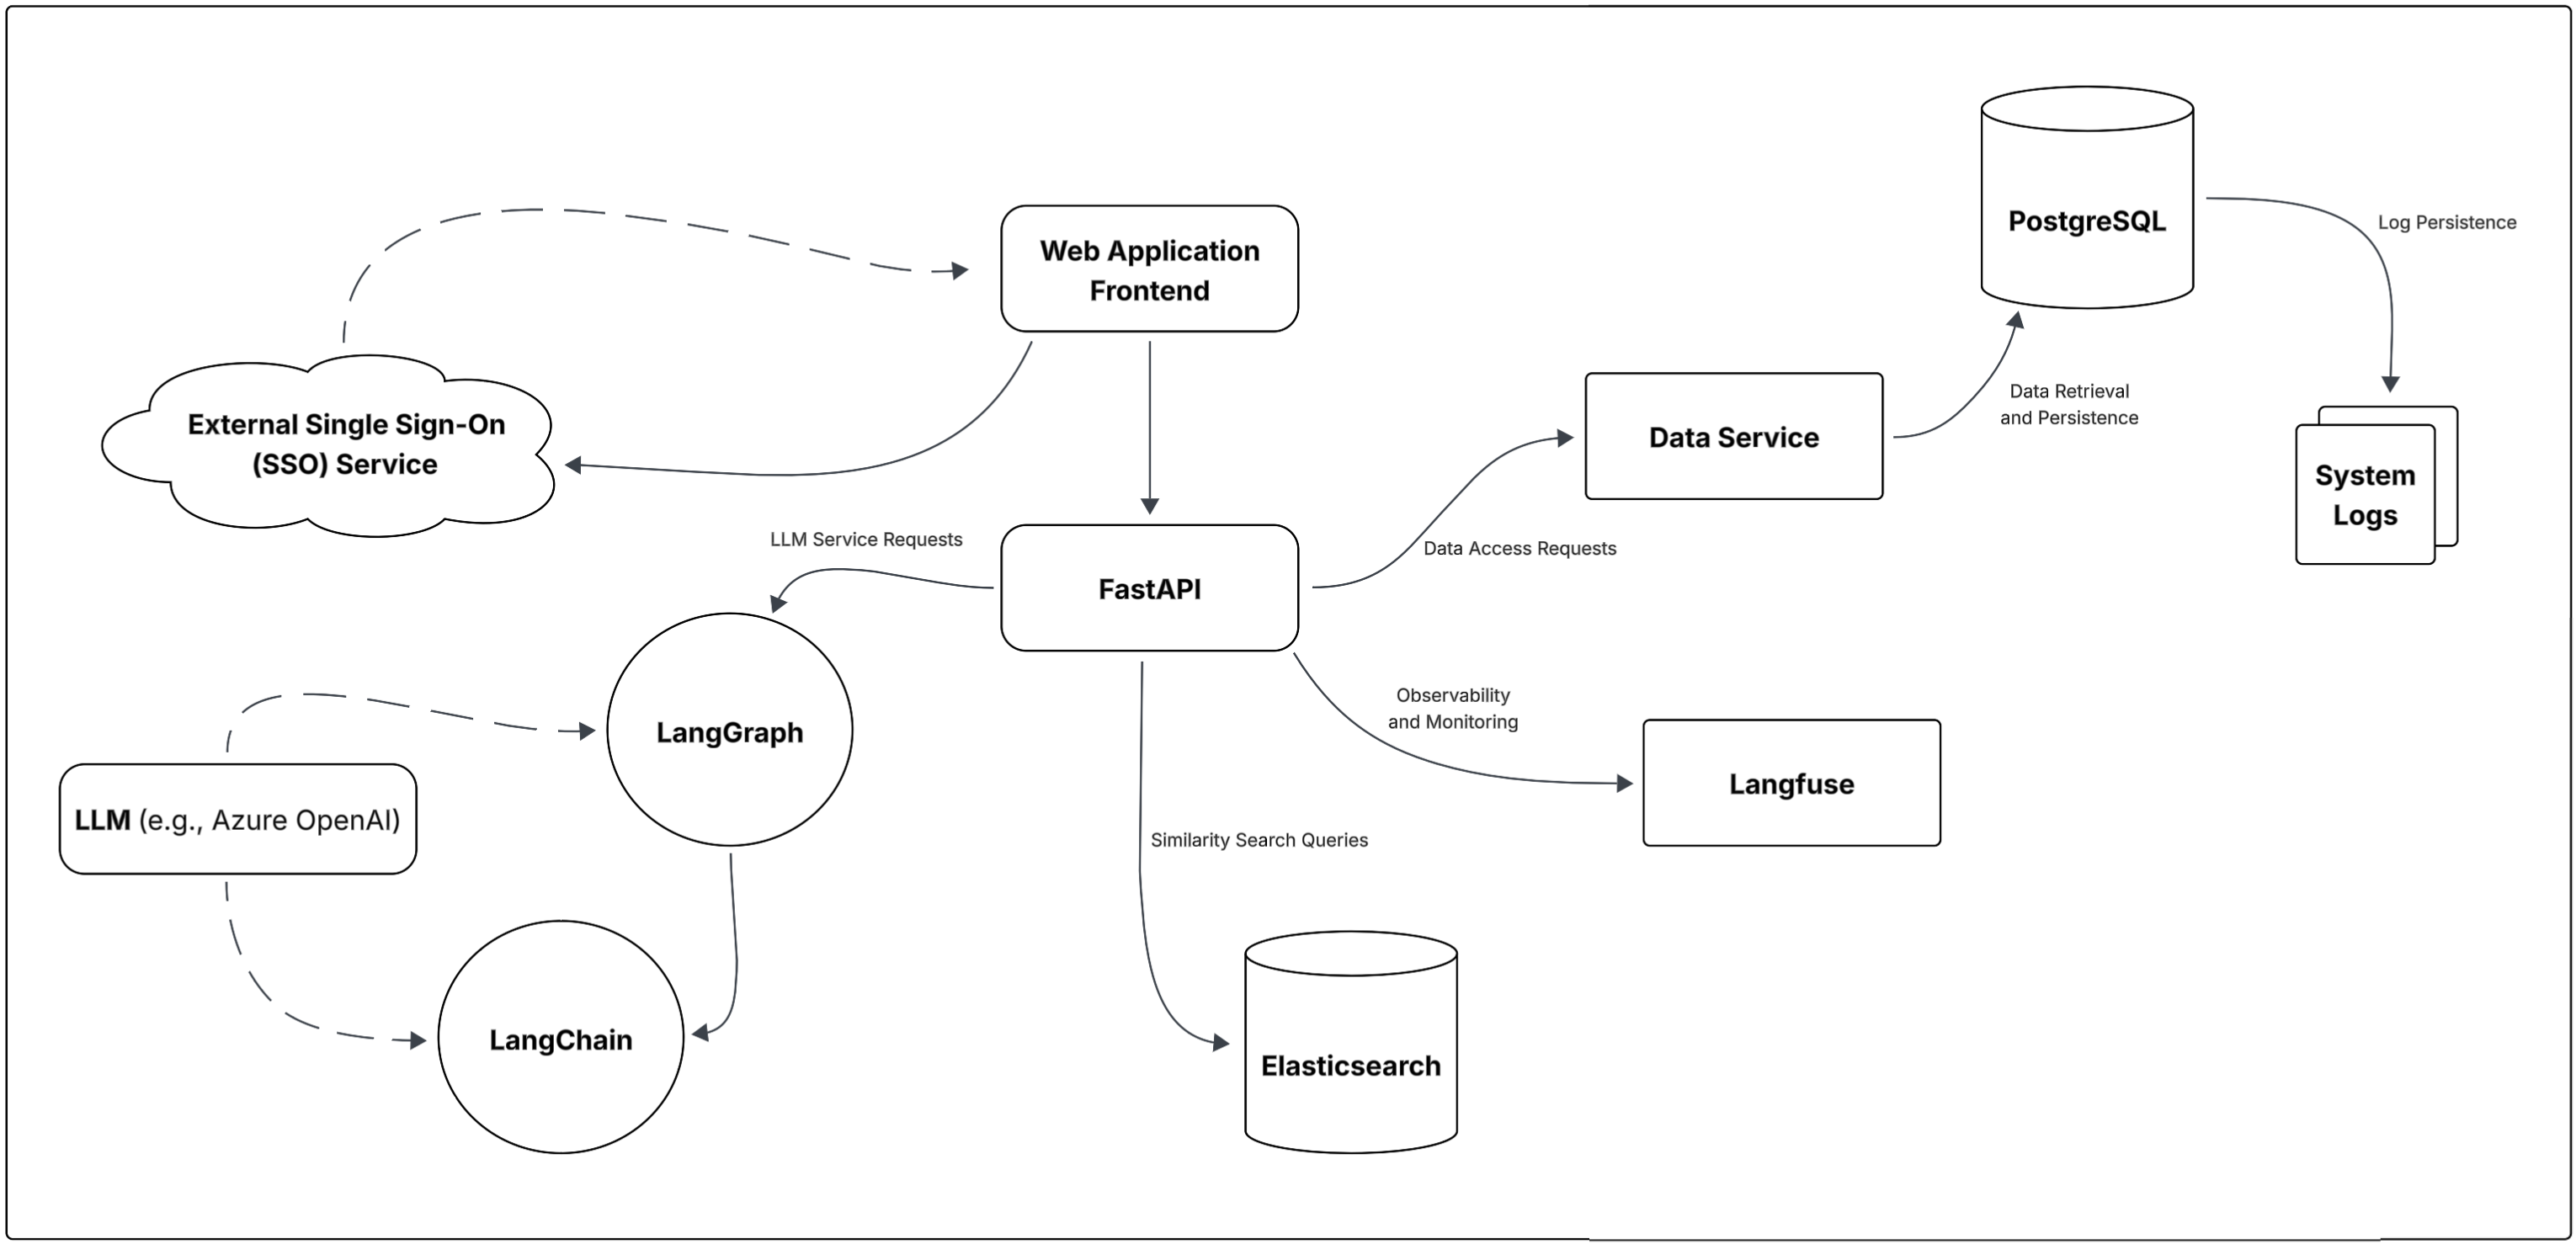
\includegraphics[width=1\textwidth]{Images/Global Architecture of the Platform.png}
    \captionof{figure}{Overall Architecture of the Platform}
    \label{fig:overall_architecture}
\end{center}

The overall architecture of the platform, as illustrated in Figure \ref{fig:overall_architecture}, depicts a structured interaction between users, frontend interfaces, backend services, databases, and AI-driven components. Users interact with the platform primarily through the web application frontend. Depending on the access requirements, users may need to authenticate via an external Single Sign-On (SSO) service to securely access private functionalities or can directly access public features like shared links through URL-based token authentication.\mynewline

The frontend communicates with the backend services built using the FastAPI framework, where the core business logic resides. This backend interacts extensively with a PostgreSQL database to persist logs and manage structured data efficiently. Elasticsearch is implemented as a vector database responsible for similarity searches, enhancing the platform’s data retrieval capabilities.\mynewline

Interaction with various Large Language Models (LLMs)—including Azure OpenAI, OpenAI GPT-4.1, and Anthropic—is managed via the LangChain framework, abstracting and simplifying communications and integration. LangGraph extends LangChain’s capabilities, facilitating the execution of complex, graph-based AI agent workflows, thereby enabling more dynamic interactions and decision-making processes within the platform.\mynewline

For observability and monitoring purposes, the system integrates Langfuse. Langfuse provides comprehensive tracking of all interactions with LLM APIs, including essential metrics such as API response times, token usage, and associated costs. This observability ensures robust management and operational transparency of the AI services integrated within the platform.

% Logical Architecture
\subsection{Logical Architecture}
This section presents the internal structure of the application codebase. Given that the core mission focused on the implementation of new features across both the backend service and frontend, the focus here will be on the logical design of these two key components.

% Main Backend Service
\subsubsection{Main Backend Service}
In the FastAPI-based backend, we adopted a layered modular architecture for each functional domain. As illustrated in Figure~\ref{fig:backend_module_architecture}, each module is composed of a controller responsible for managing HTTP and WebSocket requests, which communicates with a service layer that encapsulates the business logic. The service interacts with the data models and relies on DTOs (Data Transfer Objects) for structured data exchanges across layers.\mynewline

To abstract and streamline access to persistent storage, a DAO (Data Access Object) pattern is implemented. The DAO interfaces with a dedicated Data Service layer that encapsulates direct database operations. This clear separation of responsibilities ensures high maintainability, testability, and scalability. It also allows for improved consistency in query logic and facilitates secure data access patterns.\mynewline

This architecture was particularly beneficial for implementing legal use cases and AI-enhanced features, where the backend needed to efficiently orchestrate data retrieval, validation, and transformation between internal components and the frontend interface.

\begin{center}
    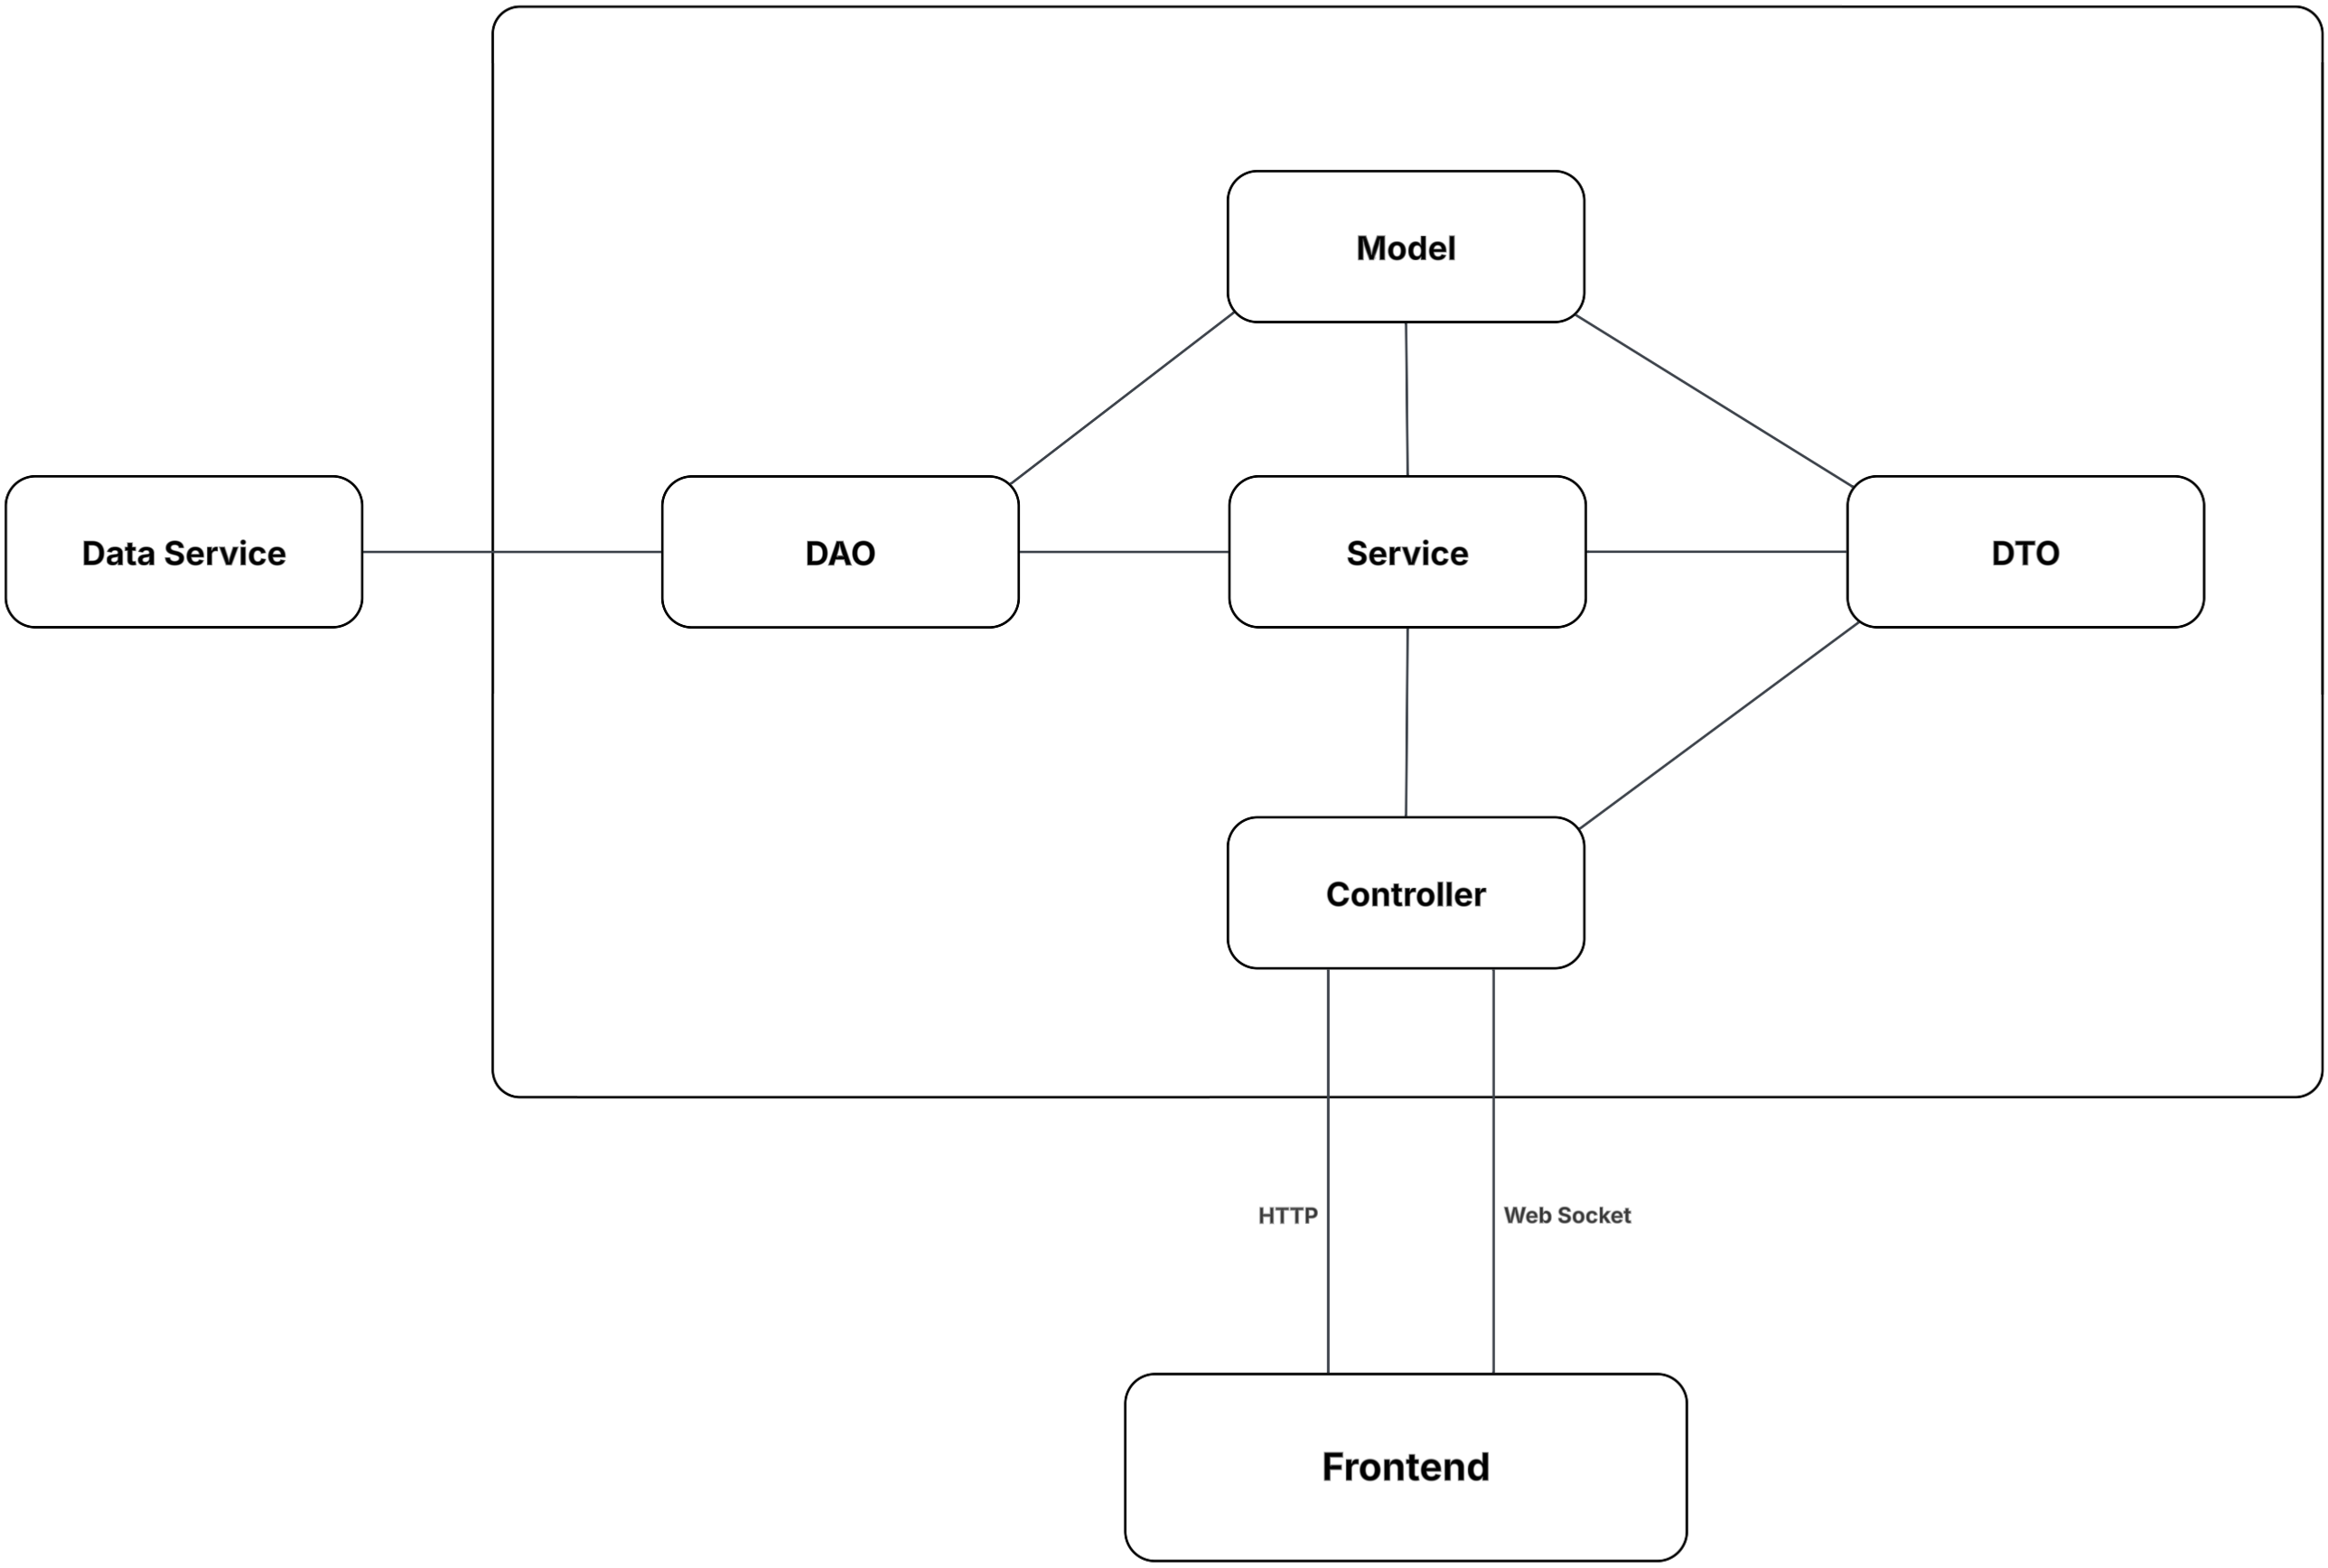
\includegraphics[width=0.95\textwidth]{Images/Layered Architecture of a Backend Module.png}
    \captionof{figure}{Layered Architecture of a Backend Module}
    \label{fig:backend_module_architecture}
\end{center}

% Frontend Structure
\subsubsection{Frontend Structure}
On the frontend side, we implemented a modular structure grounded in the principles of separation of concerns and component reusability. As shown in Figure~\ref{fig:frontend_module_architecture}, each module consists of components responsible for managing the user interface and interactions, and services that encapsulate domain-specific business logic and handle communication with the backend via HTTP or WebSocket, depending on the context.\mynewline

The architecture also integrates a dedicated store layer to manage state, especially for dynamic content and session-persistent interactions. DTOs are used to structure and validate data exchanged with the backend, while models represent the internal structure of application entities.\mynewline

This modular organization promotes code maintainability and scalability, enabling independent development and testing of each module. It also facilitates a smooth integration of new features such as AI-based clause recommendations and real-time collaboration within the contract editor.

\begin{center}
    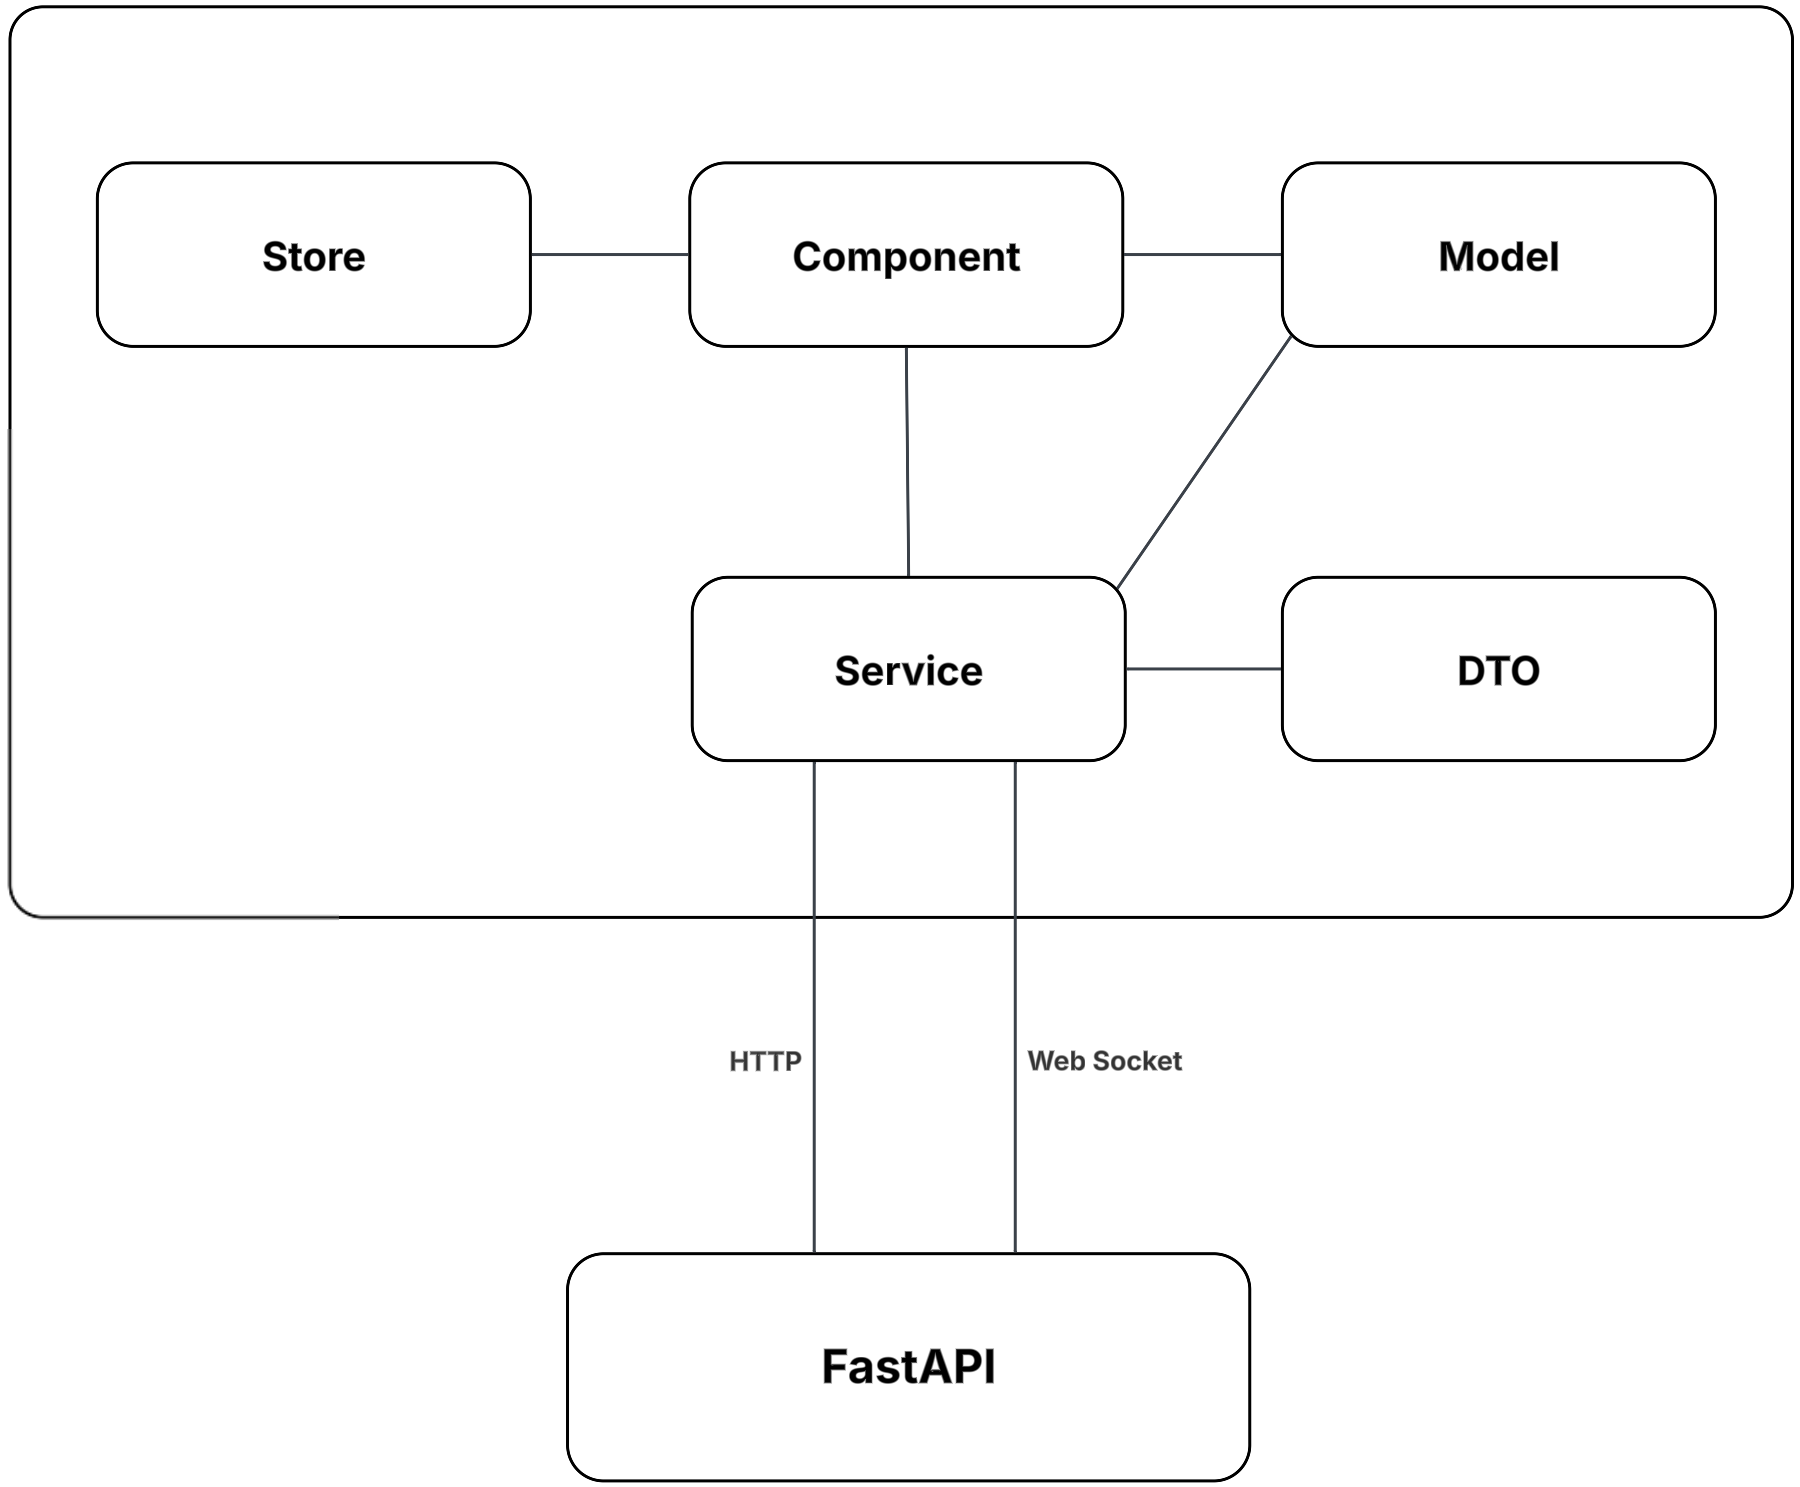
\includegraphics[width=0.95\textwidth]{Images/Component Architecture of a Frontend Module.png}
    \captionof{figure}{Component Architecture of a Frontend Module}
    \label{fig:frontend_module_architecture}
\end{center}

% LLM Integration
\subsection{LLM Integration}
Integration of LLMs within the platform is streamlined using the LangChain framework, which provides an abstraction layer to interact uniformly with multiple LLM providers. As depicted in Figure \ref{fig:llm_integration}, this integration allows the platform to remain flexible, accommodating advancements in LLM technologies with minimal architectural adjustments.\mynewline

\begin{center}
    \centering
    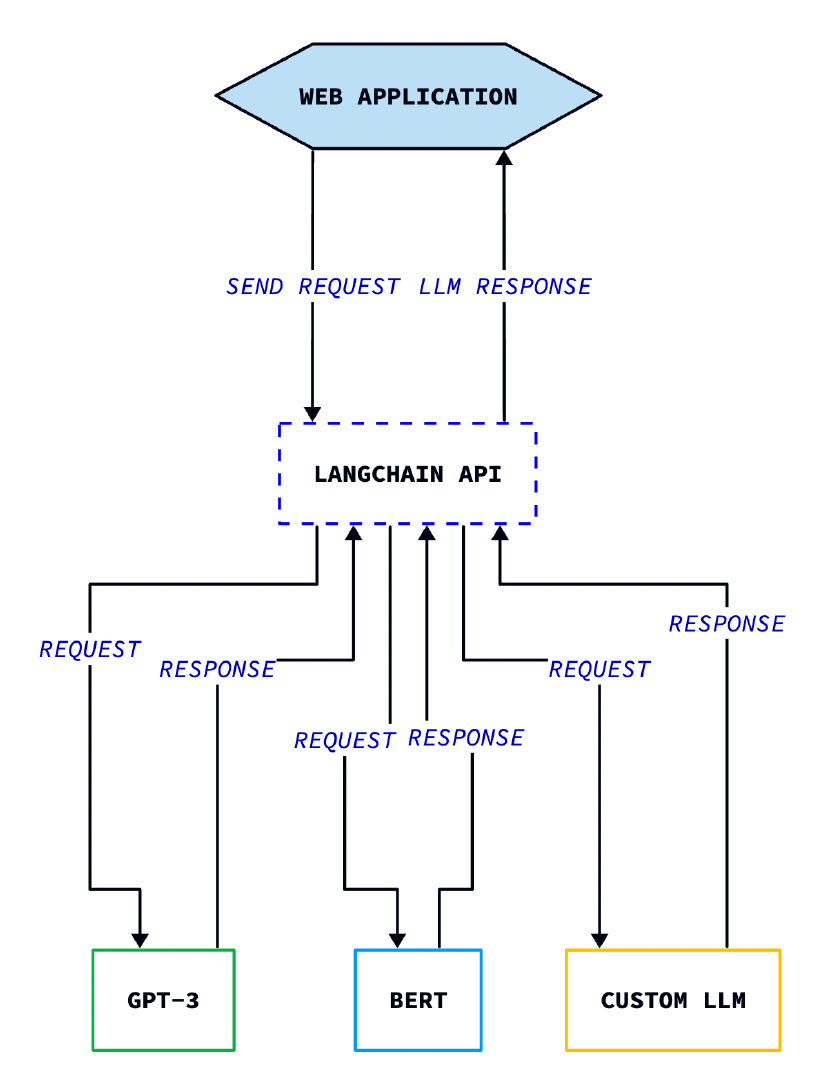
\includegraphics[width=0.6\textwidth]{Images/LLM Integration.png}
    \captionof{figure}{LLM Integration via LangChain}
    \label{fig:llm_integration}
\end{center}

LangChain efficiently manages the interaction between the platform and various LLM services, handling data flow optimization, API call management, input/output formatting, and robust error handling mechanisms. It also incorporates rate-limiting functionalities to ensure resource-efficient and cost-effective interactions.


% Text Editing Framework: Tiptap
\subsection{Text Editing Framework: Tiptap}
On the frontend, the platform employs the Tiptap editor tailored specifically for the structured editing of legal documents such as contracts. Unlike traditional rich-text editors, Tiptap is configured to meet the complex formatting and regulatory requirements intrinsic to legal documents. Users can efficiently organize document elements into legally defined sections, clauses, and subsections.\mynewline

Tiptap supports critical legal editing features, including:

\begin{itemize}
    \item \textbf{Structured Document Editing}: Customized nodes and marks for legally compliant structural elements, allowing users to efficiently manage and format contracts according to legal and organizational standards.
    \item \textbf{Clause and Variable Management}: Specialized nodes for inserting, editing, and managing clauses and dynamic contract variables directly within the document, ensuring precision and consistency.
    \item \textbf{Legal Referencing and Citations}: Dedicated support for managing legal references and citations, integrating seamlessly with internal and external legal referencing systems.
    \item \textbf{Real-time Collaborative Editing}: Integration with collaborative technologies such as Y.js enables multiple legal professionals and stakeholders to simultaneously edit, review, and approve documents, reflecting changes in real-time and maintaining a clear audit trail of modifications.
\end{itemize}

This tailored configuration of Tiptap significantly enhances the user experience, providing a robust, intuitive interface optimized specifically for drafting, reviewing, and finalizing complex legal contracts, ensuring adherence to strict legal formatting requirements.

\begin{center}
    \centering
    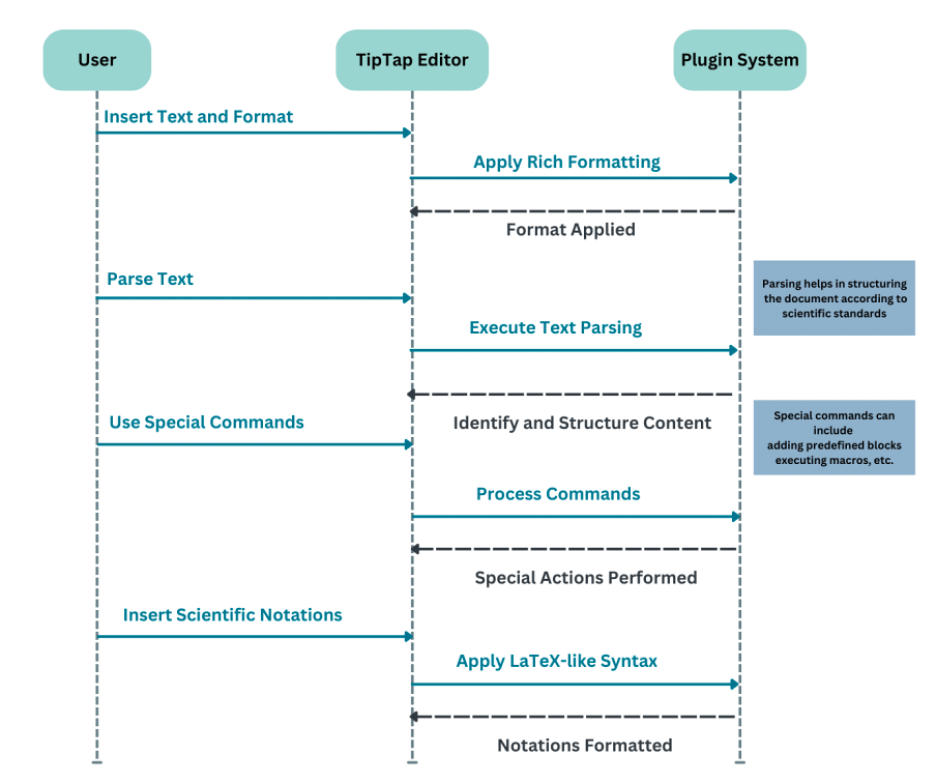
\includegraphics[width=1\textwidth]{Images/Tiptap Editing Framework.png}
    \captionof{figure}{Tiptap Text Editing Framework for Legal Documents}
    \label{fig:tiptap_legal_framework}
\end{center}


% Detailed Design
\section{Detailed Design}

% Class Diagram
\subsection{Class Diagram}
The class diagram is a fundamental UML diagram type that illustrates the static structure of the software system, detailing its classes, their attributes, methods, and the relationships among these classes. Figure \ref{fig:class_diagram} presents the comprehensive class diagram of the intelligent contract management platform developed during this internship.

\begin{center}
    \centering
    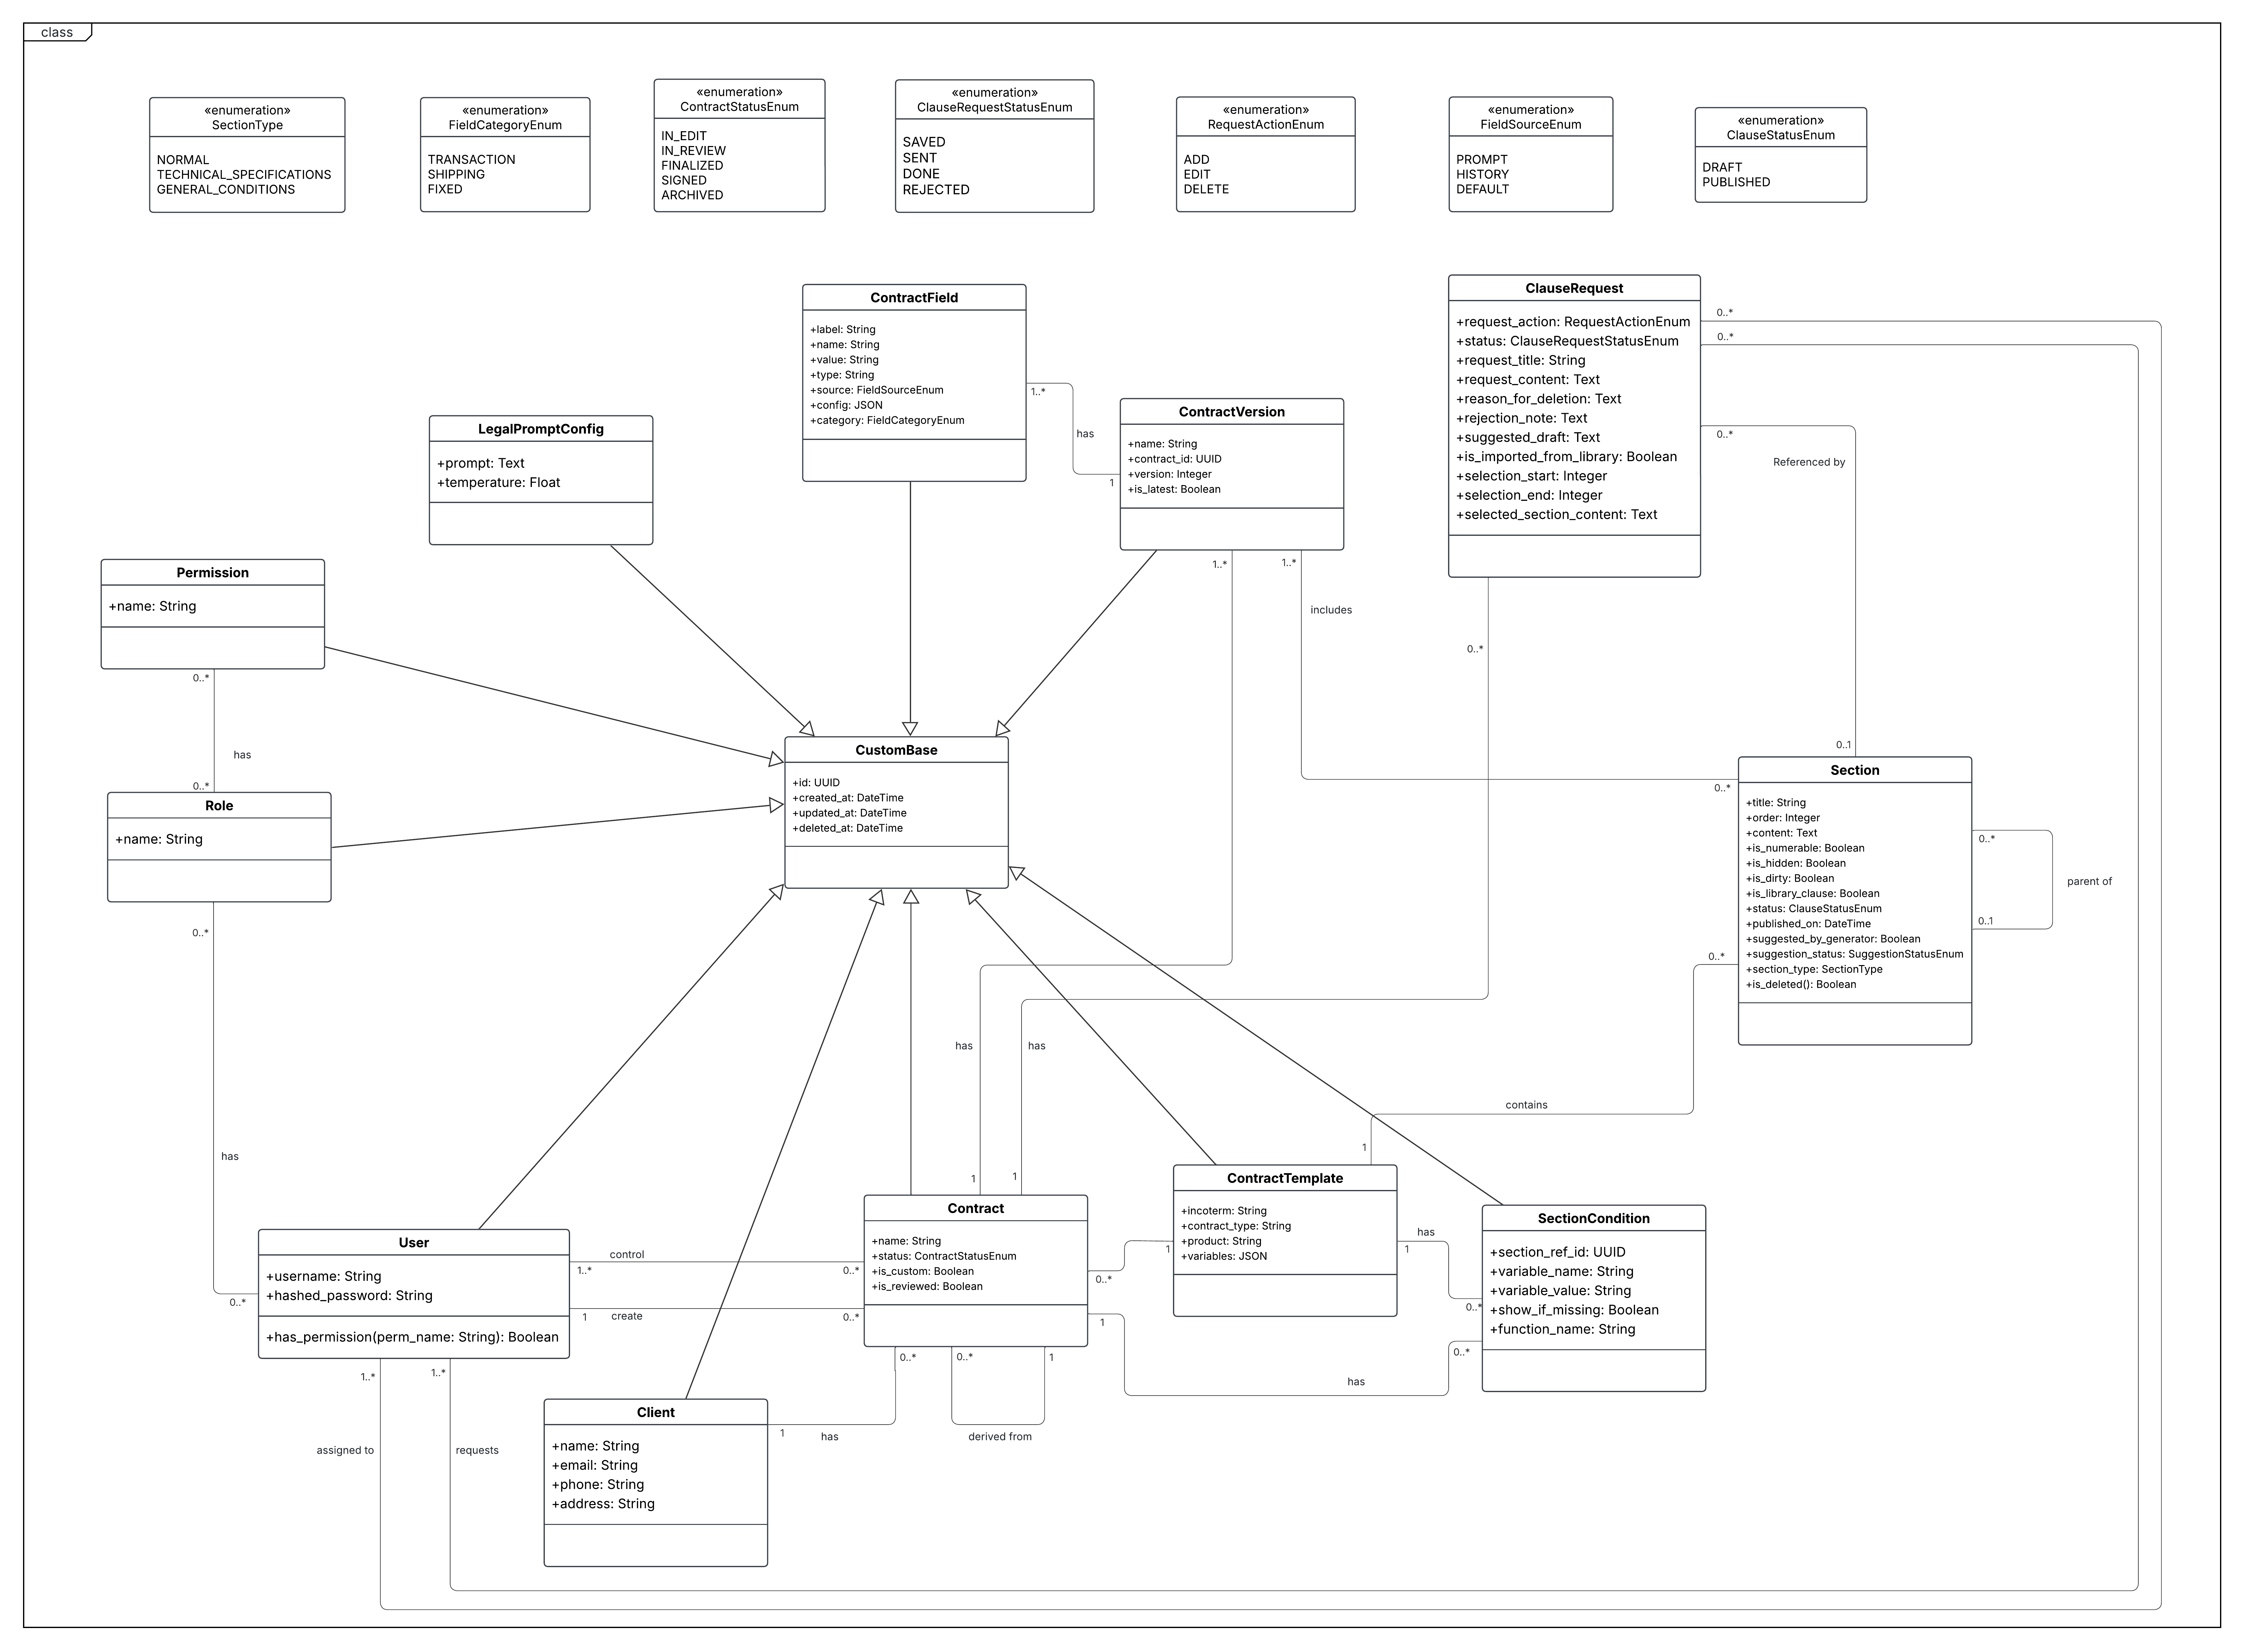
\includegraphics[width=1\textwidth]{Images/Class Diagram.png}
    \captionof{figure}{Class Diagram of The Platform}
    \label{fig:class_diagram}
\end{center}

All classes in this architecture inherit from the \textbf{CustomBase}, providing universal attributes such as a unique identifier (\textit{id}), timestamps for creation, update, and deletion of entries.\mynewline

The \textbf{User} class represents users of the platform, associating each user with specific \textbf{Roles} (e.g., Sales or Legal), which determine a set of \textbf{Permissions} defining accessible functionalities.\mynewline

The \textbf{Contract} class represents an agreement between a company and its client, distinct from the platform users. Each contract is associated with a specific \textbf{Client}, and relies on a \textbf{ContractTemplate} based on a combination of product, contract type, and Incoterm. Contracts can also originate by cloning existing contracts.\mynewline

Contracts feature five distinct statuses represented by the enumeration \textit{ContractStatusEnum}:

\begin{itemize}
    \item \textbf{IN\_EDIT}: Initial stage, editable by both Sales and Legal teams.
    \item \textbf{IN\_REVIEW}: Editable by Legal, but frozen for Sales, acting as a proxy to finalization.
    \item \textbf{FINALIZED}: Fully reviewed and locked from editing by both teams.
    \item \textbf{SIGNED}: Confirmed and mutually agreed upon by the company and the client.
    \item \textbf{ARCHIVED}: Used for historical purposes based on the company's archiving policies.
\end{itemize}

Each \textbf{Contract} is composed of one or multiple \textbf{ContractVersions} to manage iterative changes and improvements. Versions include structured \textbf{Sections}, each comprising multiple fields detailed by \textbf{ContractField} classes representing variables specific to each contract section.\mynewline

The \textbf{ClauseRequest} class is specifically dedicated to handling clause modification requests made by Sales users to the Legal team, marked by statuses within the \textit{ClauseRequestStatusEnum} (\textit{SAVED}, \textit{SENT}, \textit{DONE}, \textit{REJECTED}). Requests transition from \textit{SAVED} when initially drafted by a Sales user, to \textit{SENT} upon submission to Legal. Depending on the decision by Legal, these requests become \textit{DONE} upon acceptance and implementation, or \textit{REJECTED} if not approved.\mynewline

This class diagram provides a clear and structured representation, highlighting crucial entities, their interrelations, and functionalities integral to the platform’s effective management of digital contract operations.


% Detailed Sequence Diagram
\subsection{Detailed Sequence Diagram}
Following the analysis phase where chronological interactions between the system and actors were outlined, detailed sequence diagrams have been created. These diagrams precisely illustrate interactions among system components to realize specific use cases. The use cases chosen for detailed representation are \textbf{Generate a New Contract}, \textbf{Create Clause Request} and \textbf{Review Clause Request}.

% Generate a New Contract
\subsubsection{Generate a New Contract}

\begin{center}
    \centering
    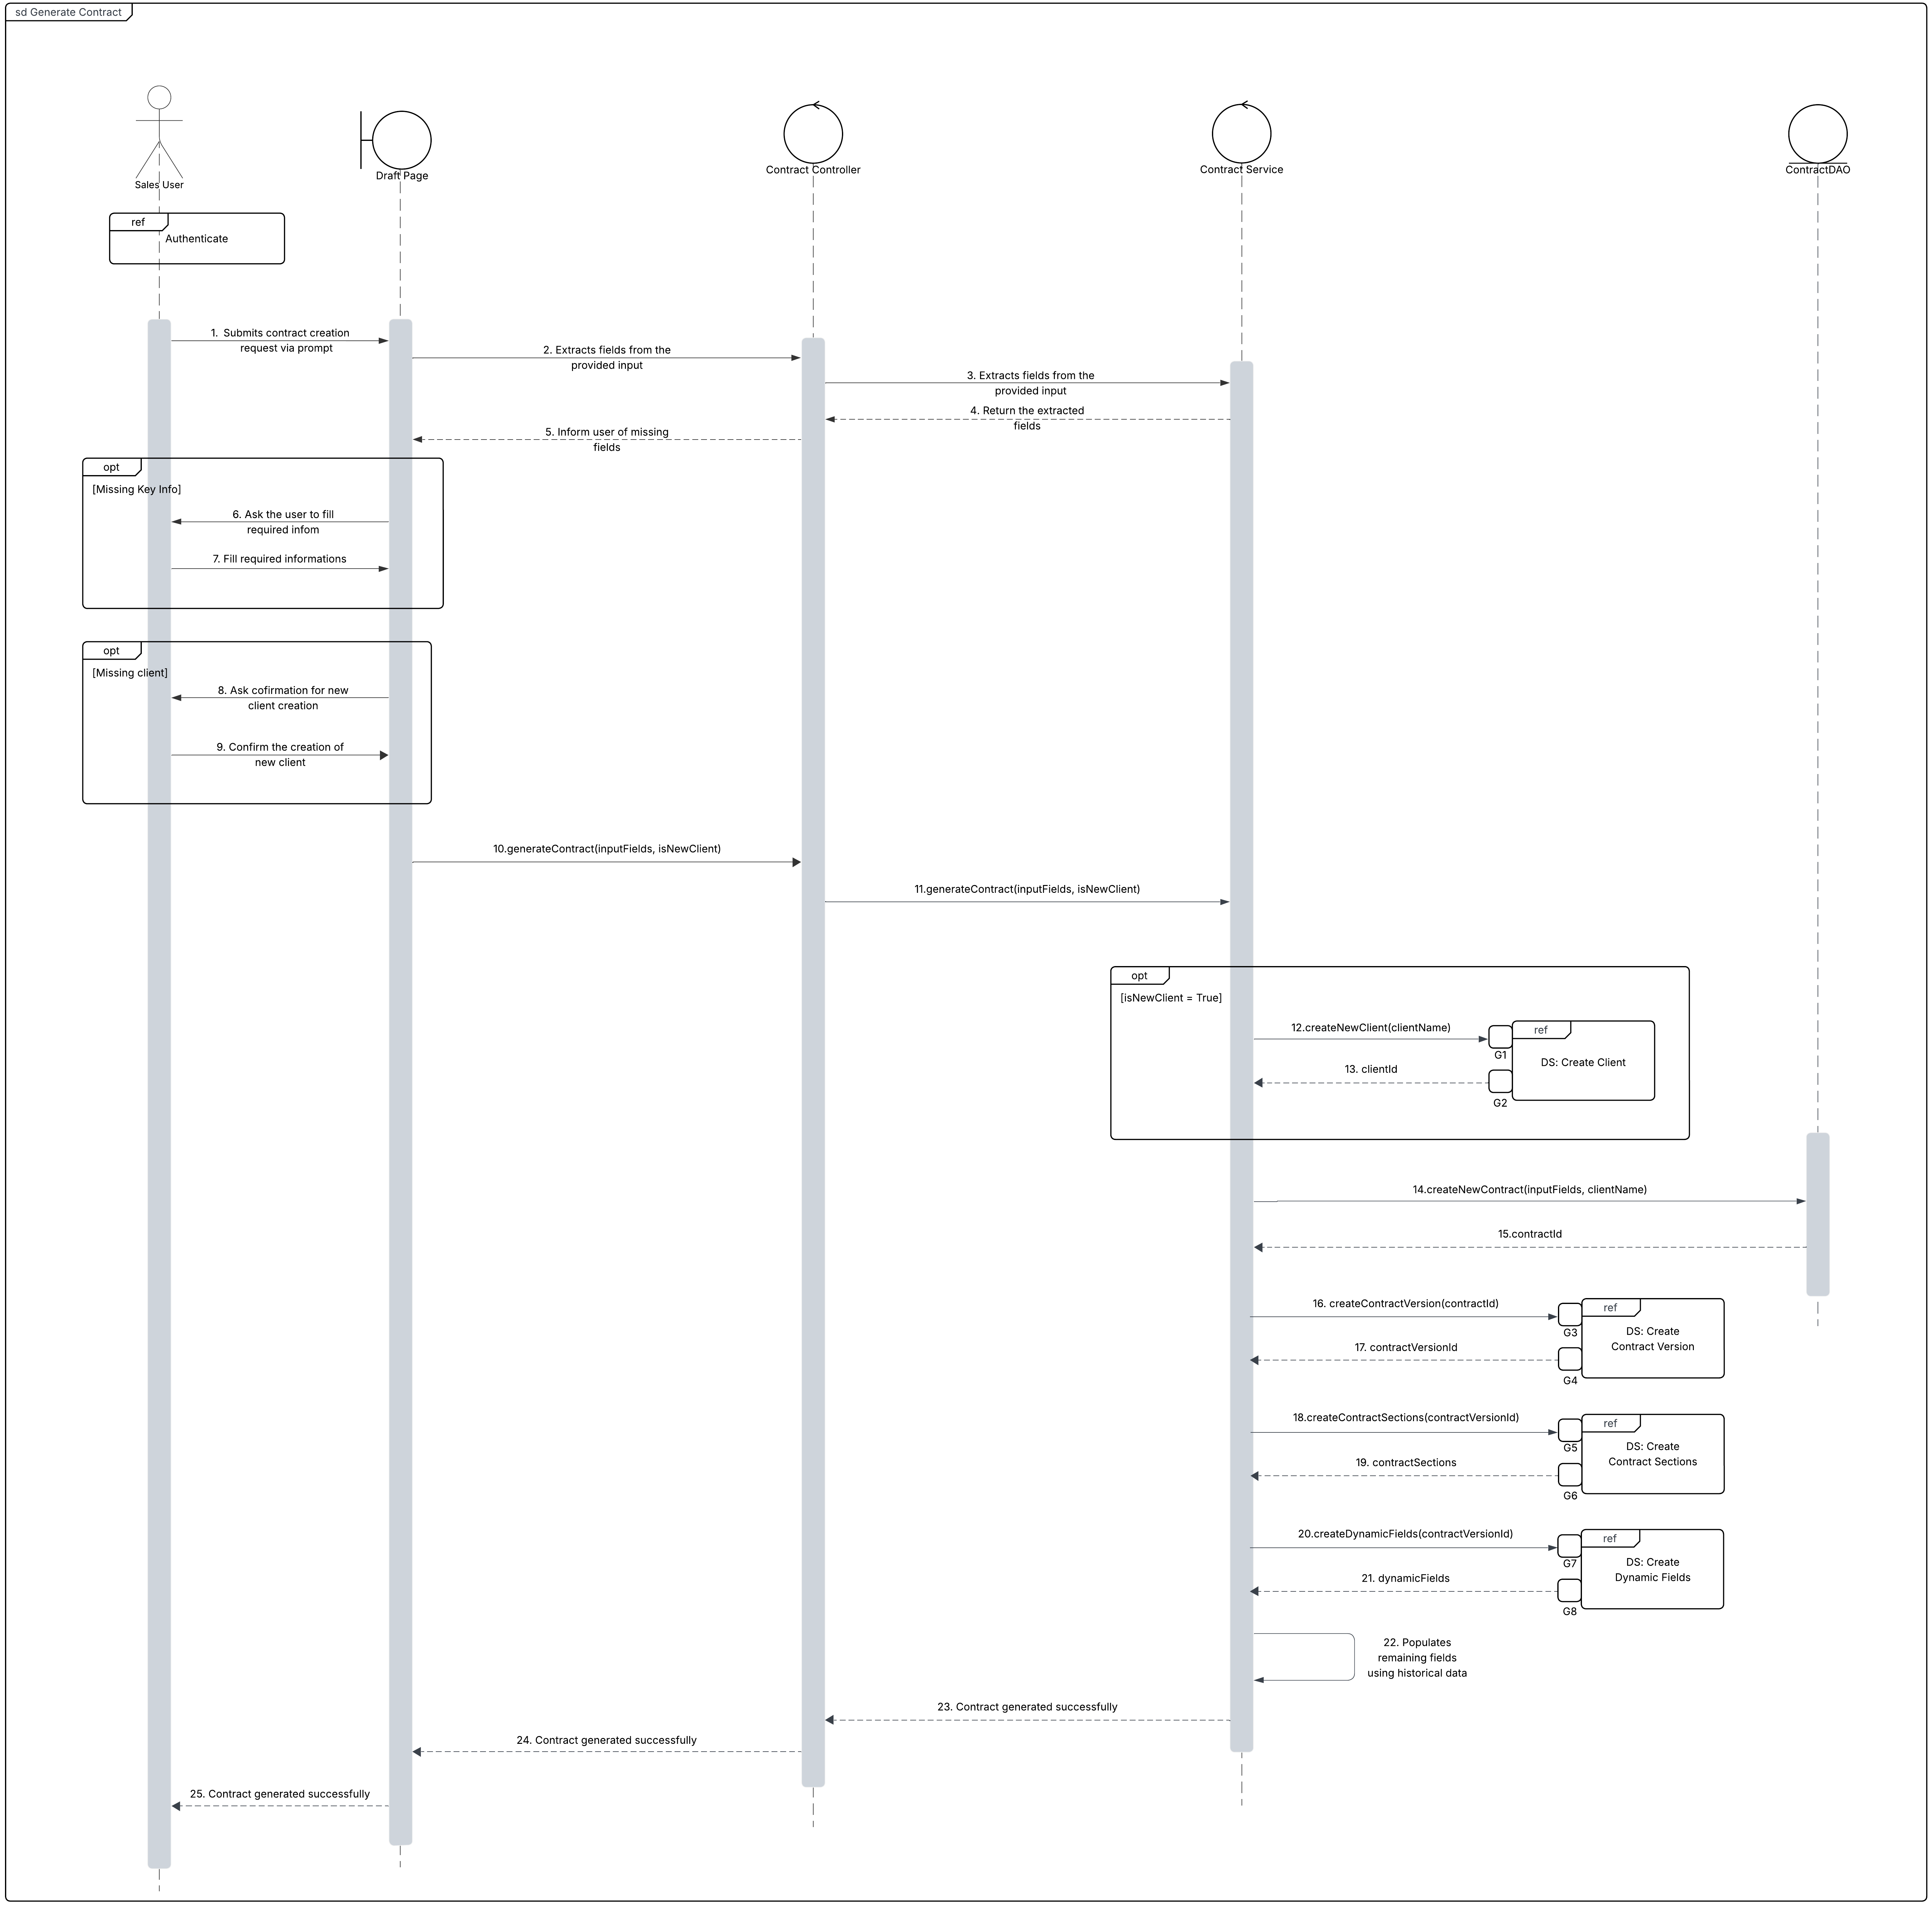
\includegraphics[width=1\textwidth]{Images/Sequence Diagram - Draft Contract.png}
    \captionof{figure}{Sequence Diagram - Draft Contract}
    \label{fig:sequence_diagram_draft_contract}
\end{center}

Figure \ref{fig:sequence_diagram_draft_contract} depicts the detailed sequence diagram for generating a new contract. In this scenario, the sales user initiates by logging into the system and providing a prompt through text, voice, or image, detailing essential information needed for the contract. The system then extracts necessary fields such as Incoterm, contract type, product, and client name to identify the appropriate template and client data. If critical information is missing or a new client is identified, the system prompts the user for clarification or confirmation to avoid mismatches.\mynewline

Upon confirmation, the system creates a new client record if necessary, extracts dynamic fields from the provided prompt, selects the appropriate contract template, and populates the dynamic fields accordingly. Missing fields are filled either by referencing a specific past contract indicated by the user or by defaulting to the client's most recent contract. If the client is new or no relevant contracts are found, fields remain empty. After contract generation, the user is automatically redirected to the contract editing interface.

% Clause Request Lifecycle
\subsubsection{Clause Request Lifecycle}

The Clause Request Lifecycle involves coordinated interactions between sales and legal teams, as shown in Figure \ref{fig:sequence_diagram_clause_request_sales} and Figure \ref{fig:sequence_diagram_clause_request_legal}. Initially, a sales user creates a clause request by providing a description for modifying, adding, or deleting clauses within a contract. The user can optionally refine this description with assistance from the Refiner Agent, which leverages an LLM to enhance clarity and precision. The sales user can then either save the request for later or send it directly to the legal team.\mynewline

Upon submission, the legal team receives a notification of the new clause request. Legal users may reject the request immediately by providing specific feedback or accept it for further processing. Accepted requests prompt legal users to utilize a dedicated editor to craft or modify clauses as requested. Completed clauses may be directly integrated into the active contract by publishing, or saved in the clause library for future use.

\begin{center}
    \centering
    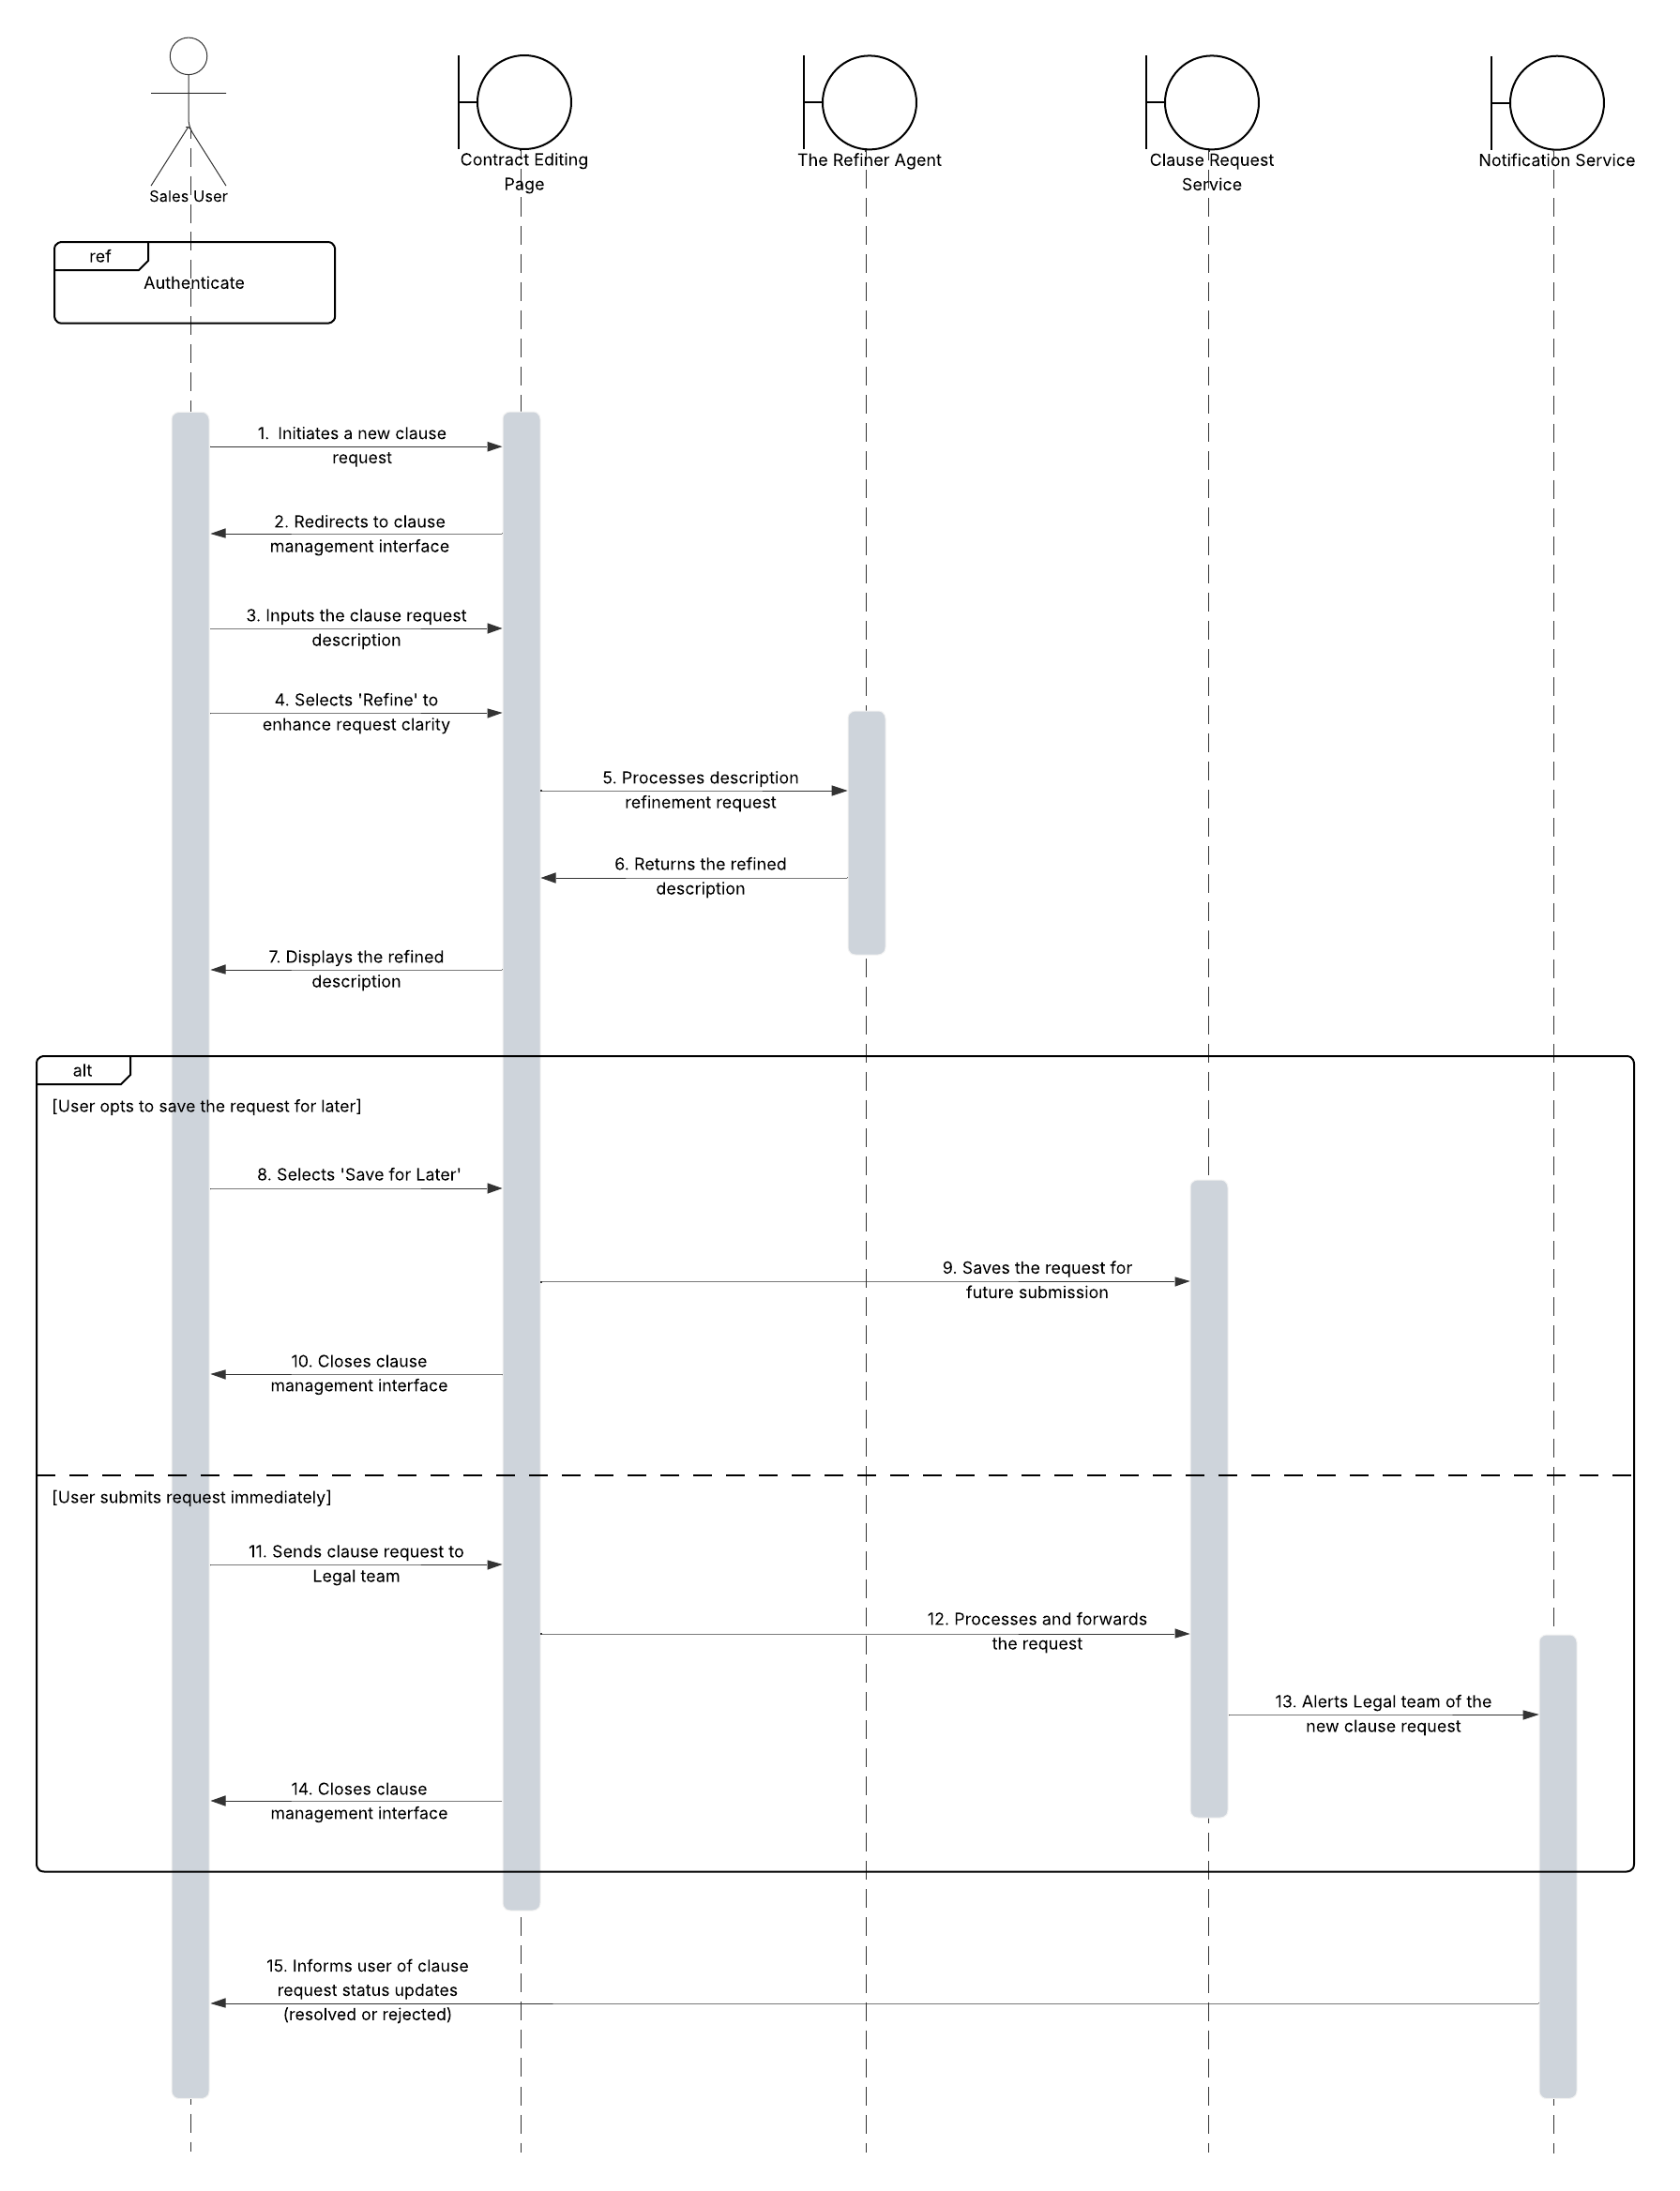
\includegraphics[width=1\textwidth]{Images/Sequence Diagram - Sales - Clause Request.png}
    \captionof{figure}{Sequence Diagram - Clause Request (Sales Perspective)}
    \label{fig:sequence_diagram_clause_request_sales}
\end{center}

\begin{center}
    \centering
    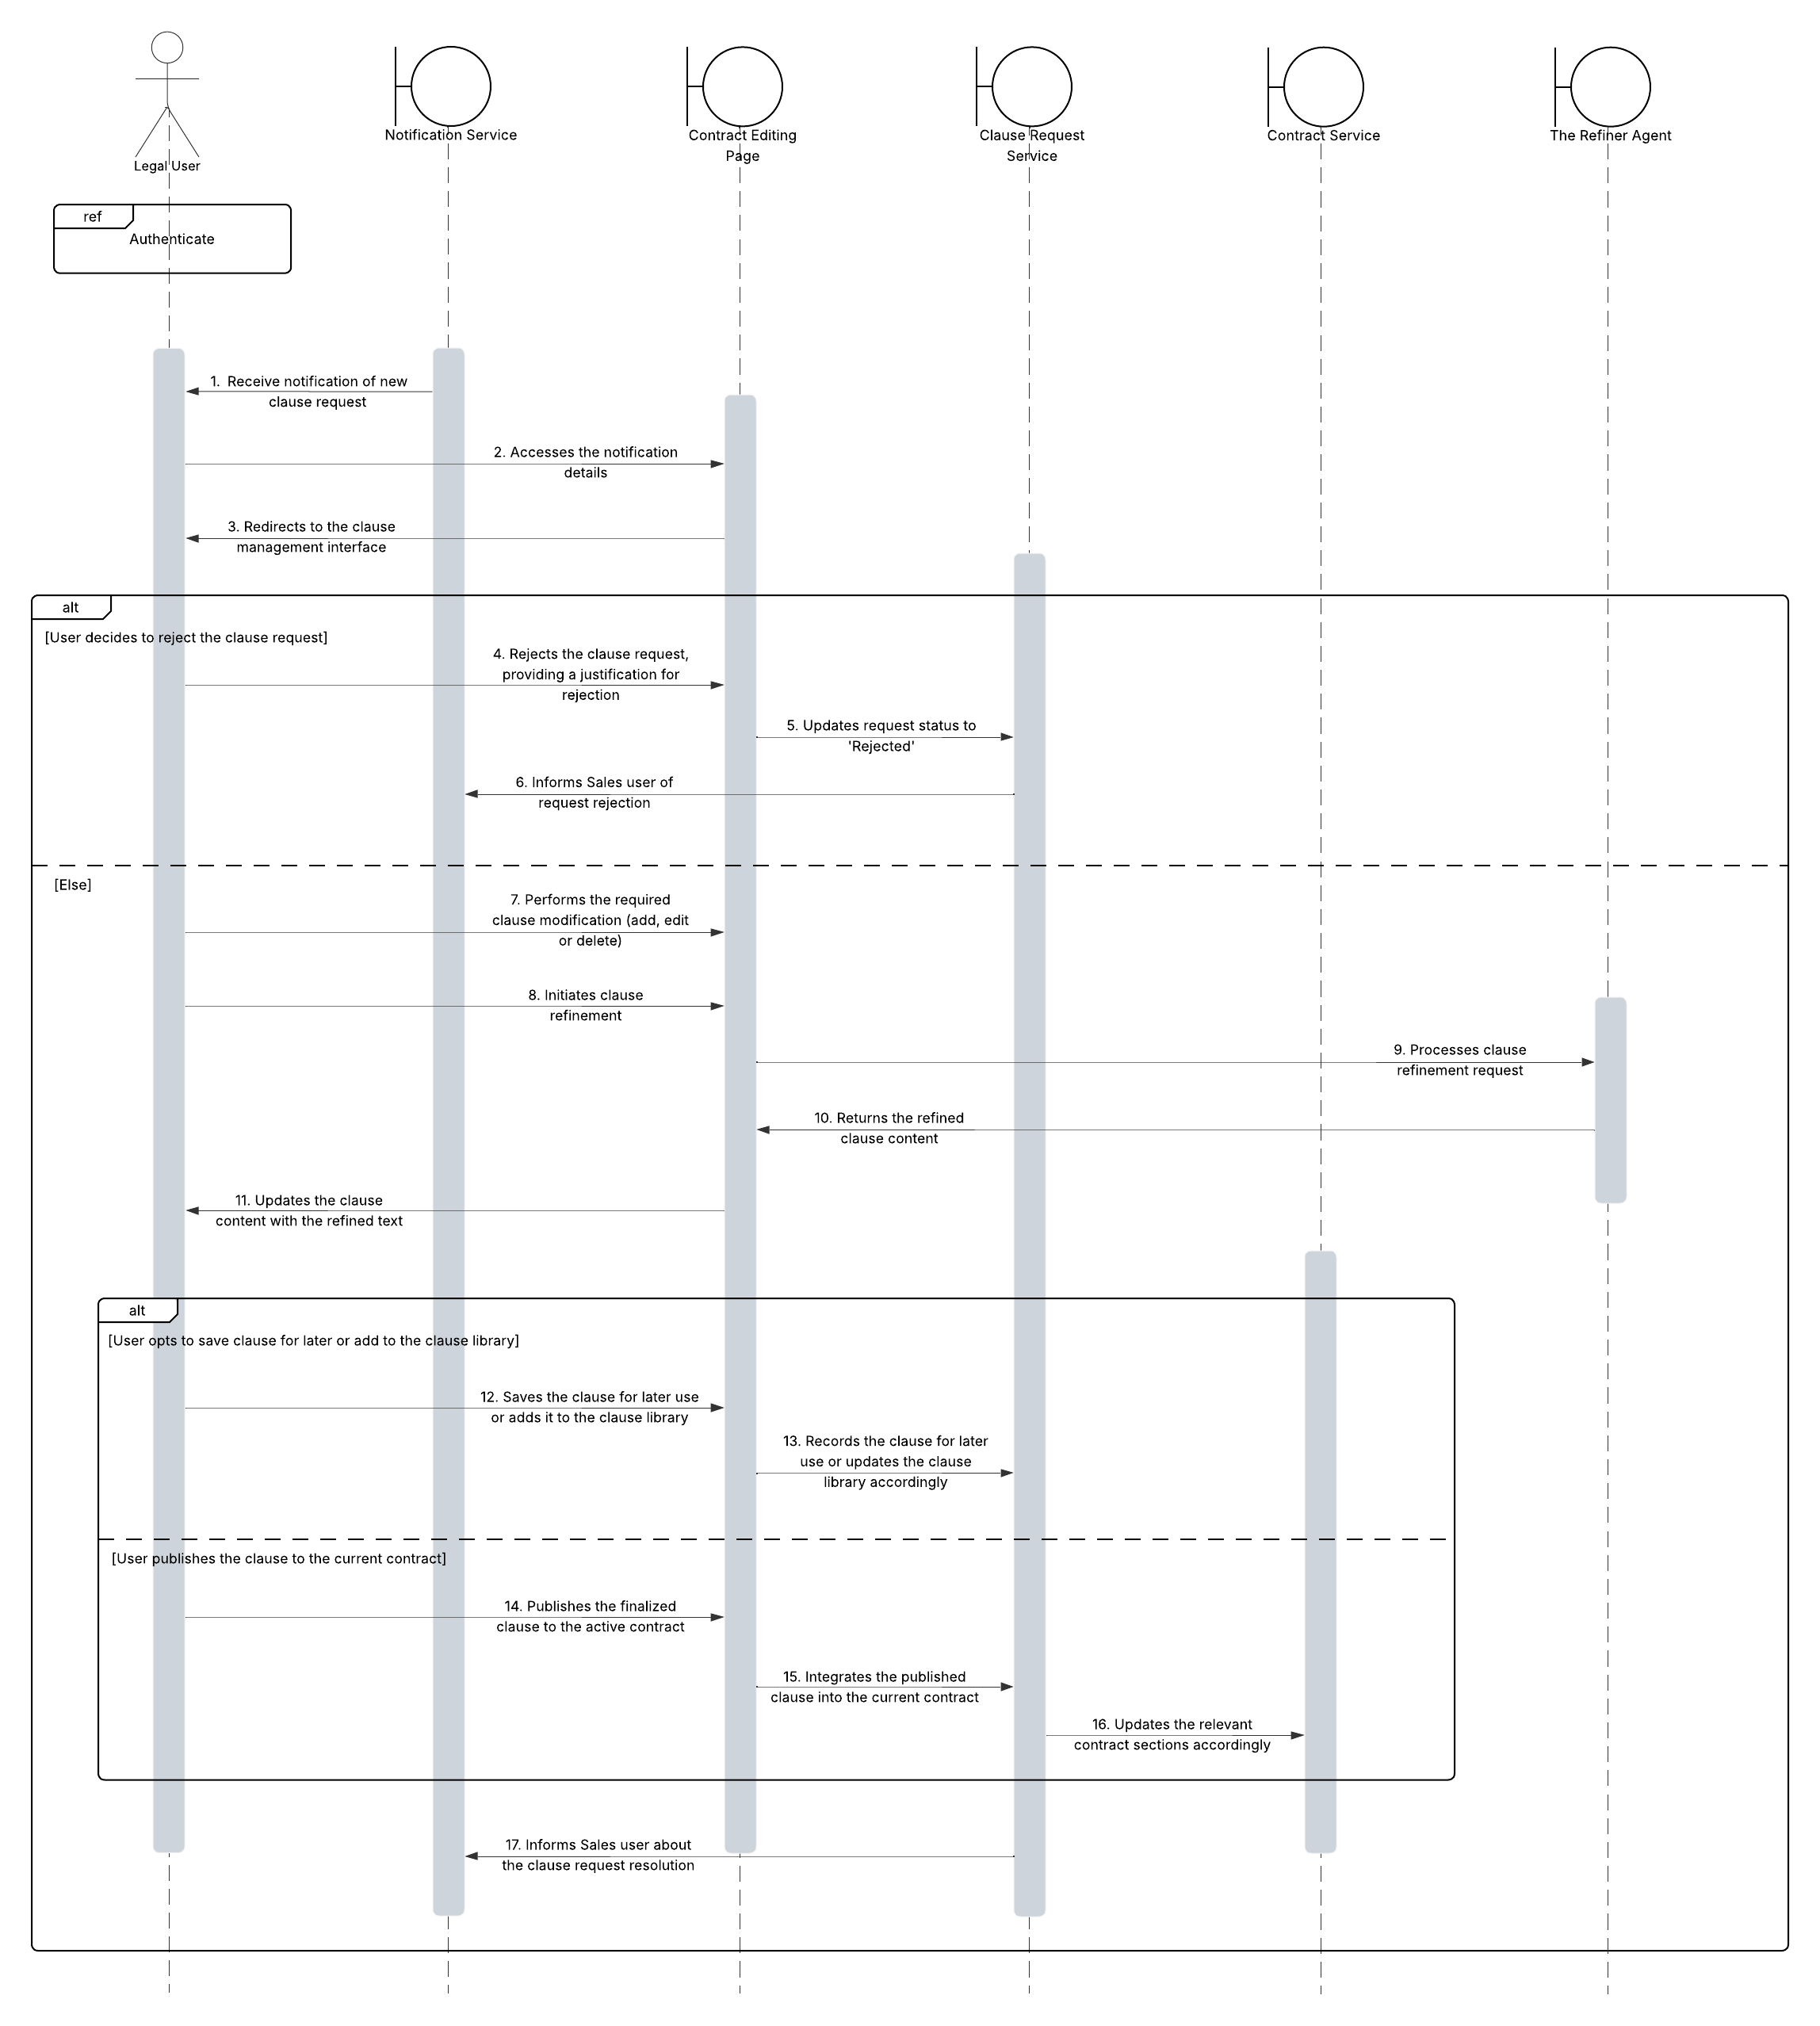
\includegraphics[width=1\textwidth]{Images/Sequence Diagram - Legal - Clause Request.png}
    \captionof{figure}{Sequence Diagram - Clause Request (Legal Perspective)}
    \label{fig:sequence_diagram_clause_request_legal}
\end{center}

These diagrams comprehensively clarify the interactions between system components, highlighting critical processes and dependencies to ensure a smooth and efficient workflow within the intelligent contract management platform.

% Technical and Deployment Architectures
\section{Technical and Deployment Architectures}

% Infrastructure Architecture
\subsection{Infrastructure Architecture}
The infrastructure architecture provides a robust foundation leveraging Microsoft Azure, optimized for scalability, security, and high performance. This architecture is strategically structured into three primary layers: compute and deployment, networking and API management, and storage and data management, as illustrated in Figure \ref{fig:infra_architecture}.

\begin{center}
    \centering
    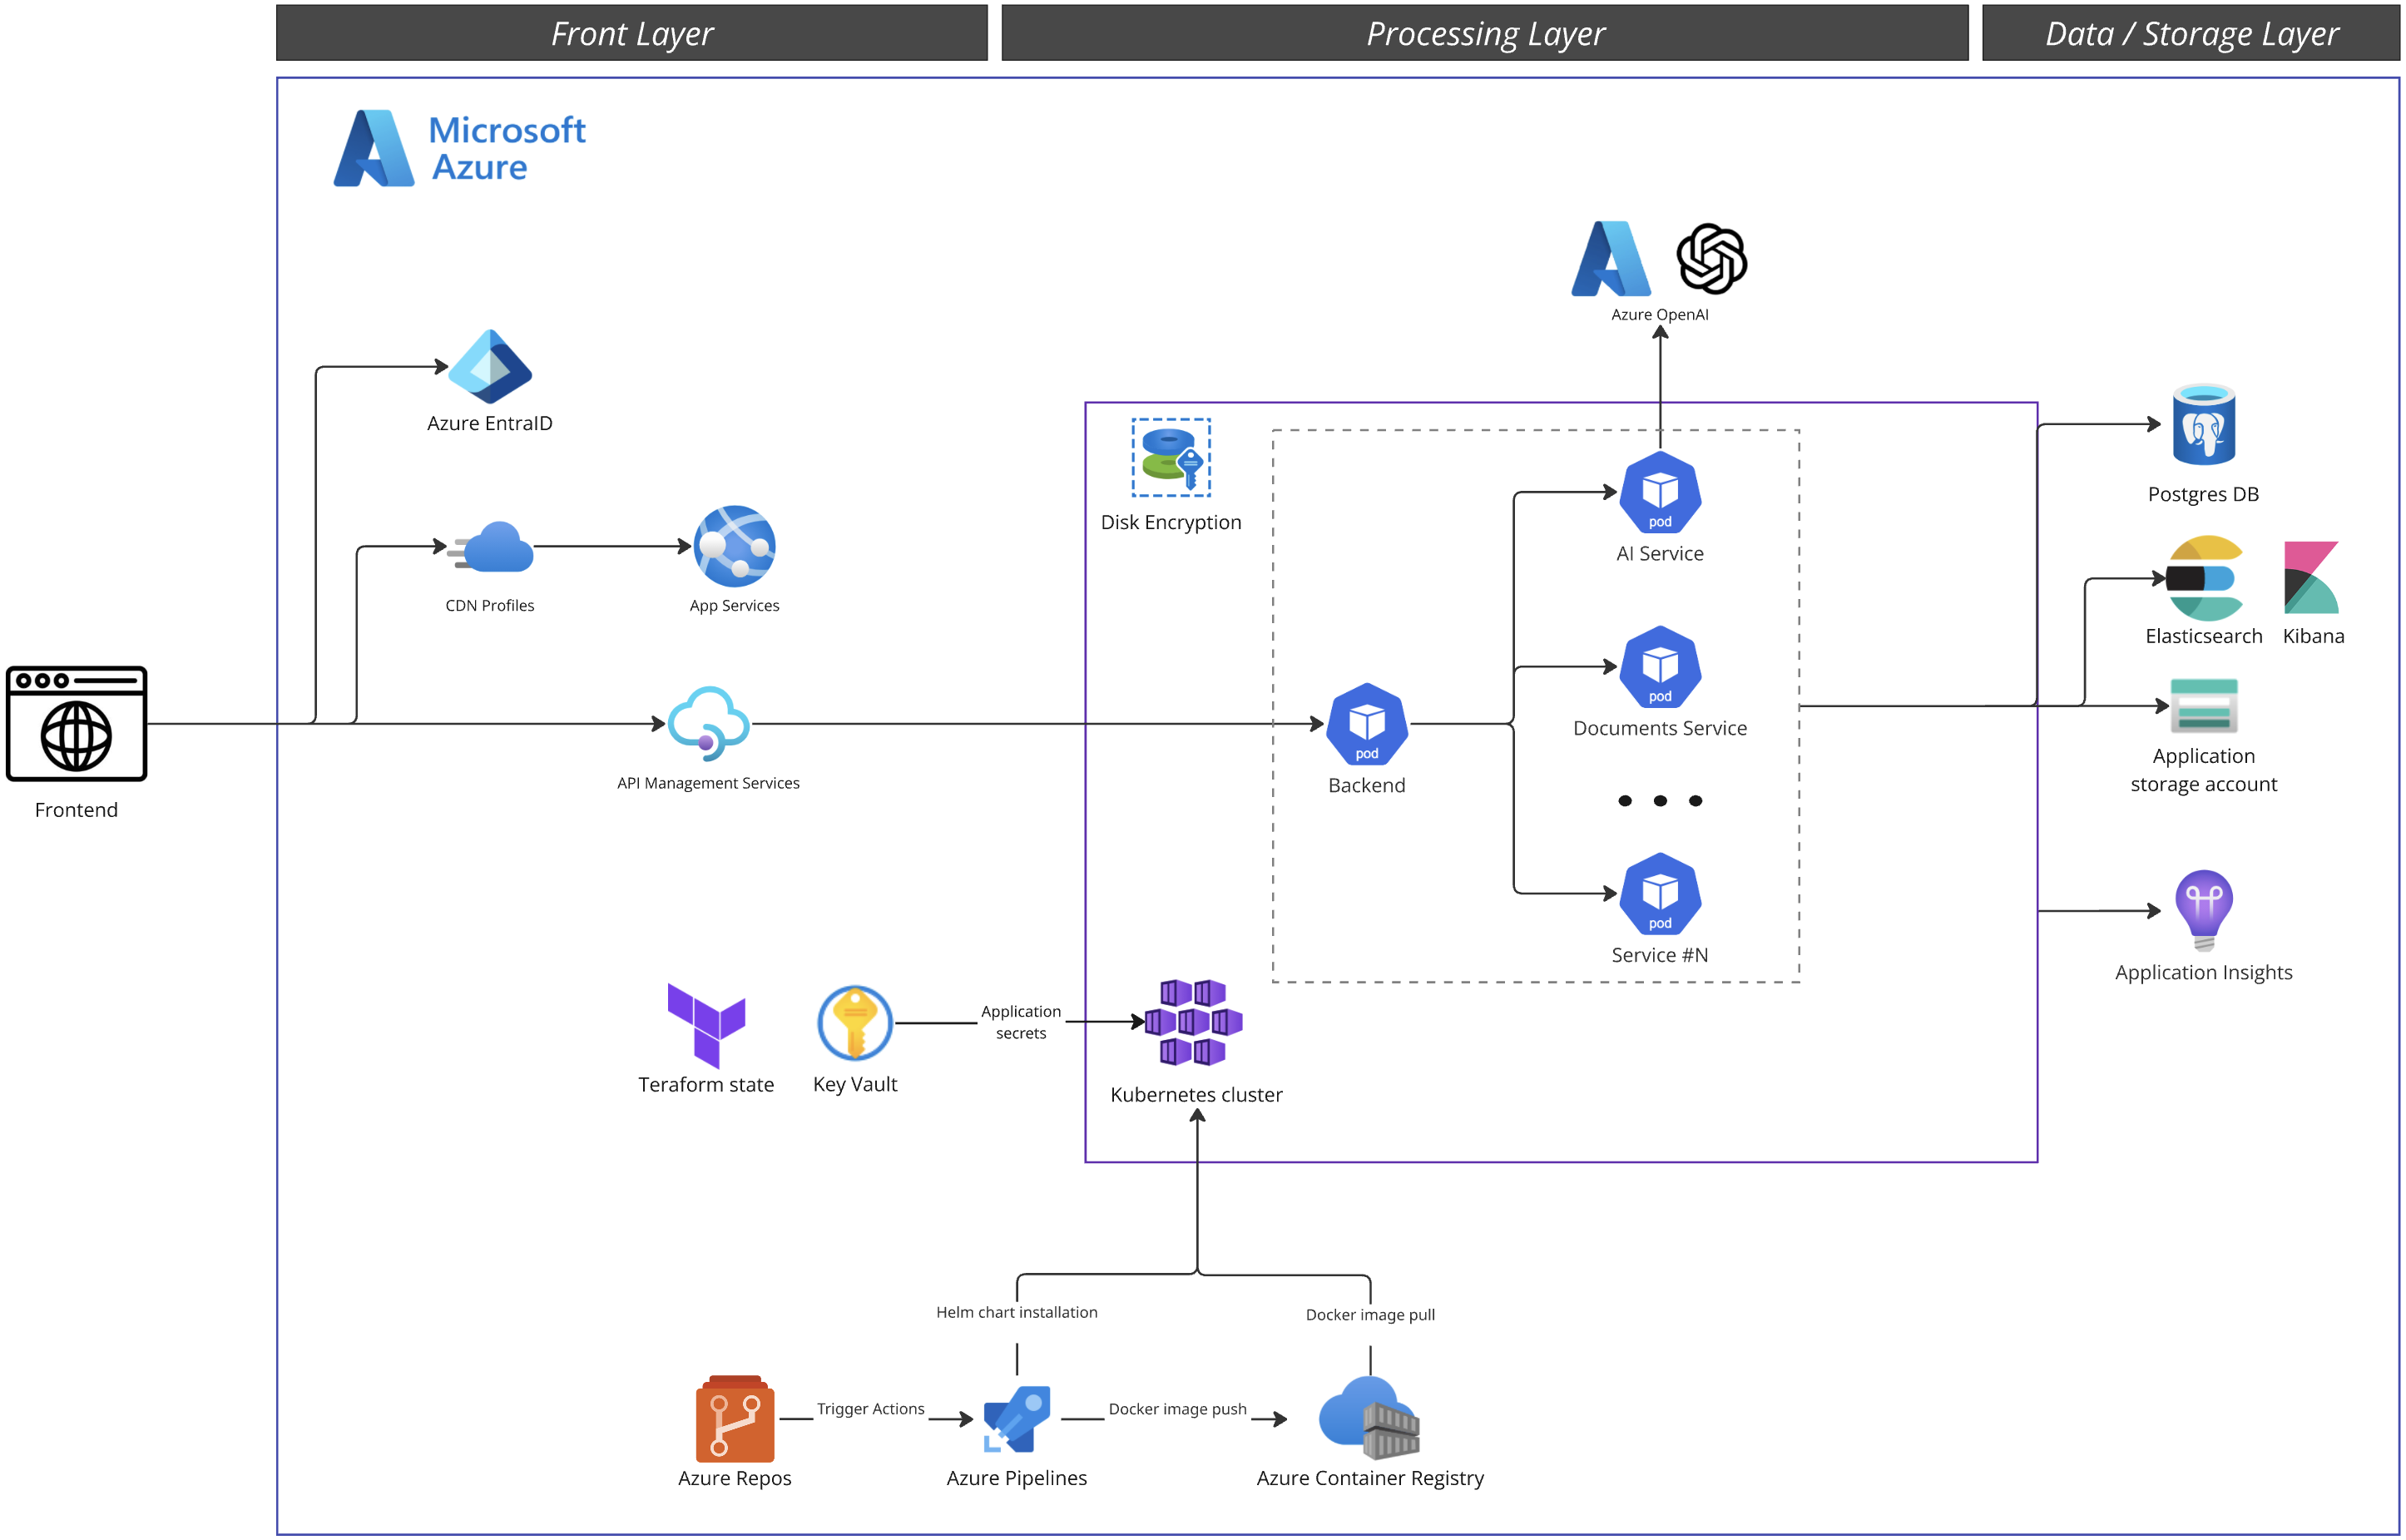
\includegraphics[width=1\textwidth]{Images/Infra Architecture.png}
    \captionof{figure}{Infrastructure Architecture Overview}
    \label{fig:infra_architecture}
\end{center}

Azure Kubernetes Service (AKS) manages containerized workloads, ensuring auto-scaling, self-healing, and smooth rolling deployments. The frontend is efficiently hosted using Azure App Services, benefiting from dynamic scaling and easy CI/CD integration. Azure API Management acts as a secure gateway managing API interactions, implementing policies, and providing rate limiting. Networking security is further reinforced by Azure Virtual Networks (VNet) and enhanced performance through Azure Content Delivery Network (CDN). Azure Blob Storage supports unstructured data, while Azure PostgreSQL and Elasticsearch with Kibana manage structured data, ensuring efficient data storage and retrieval. Security, observability, and automation are seamlessly integrated through Azure Key Vault, Azure Disk Encryption, Azure Monitor, Application Insights, Terraform, and Helm.

% Security Architecture
\subsection{Security Architecture}
Security architecture ensures comprehensive protection against threats, maintaining data integrity, confidentiality, and secure communications, as shown in Figure \ref{fig:security_architecture}.

\begin{center}
    \centering
    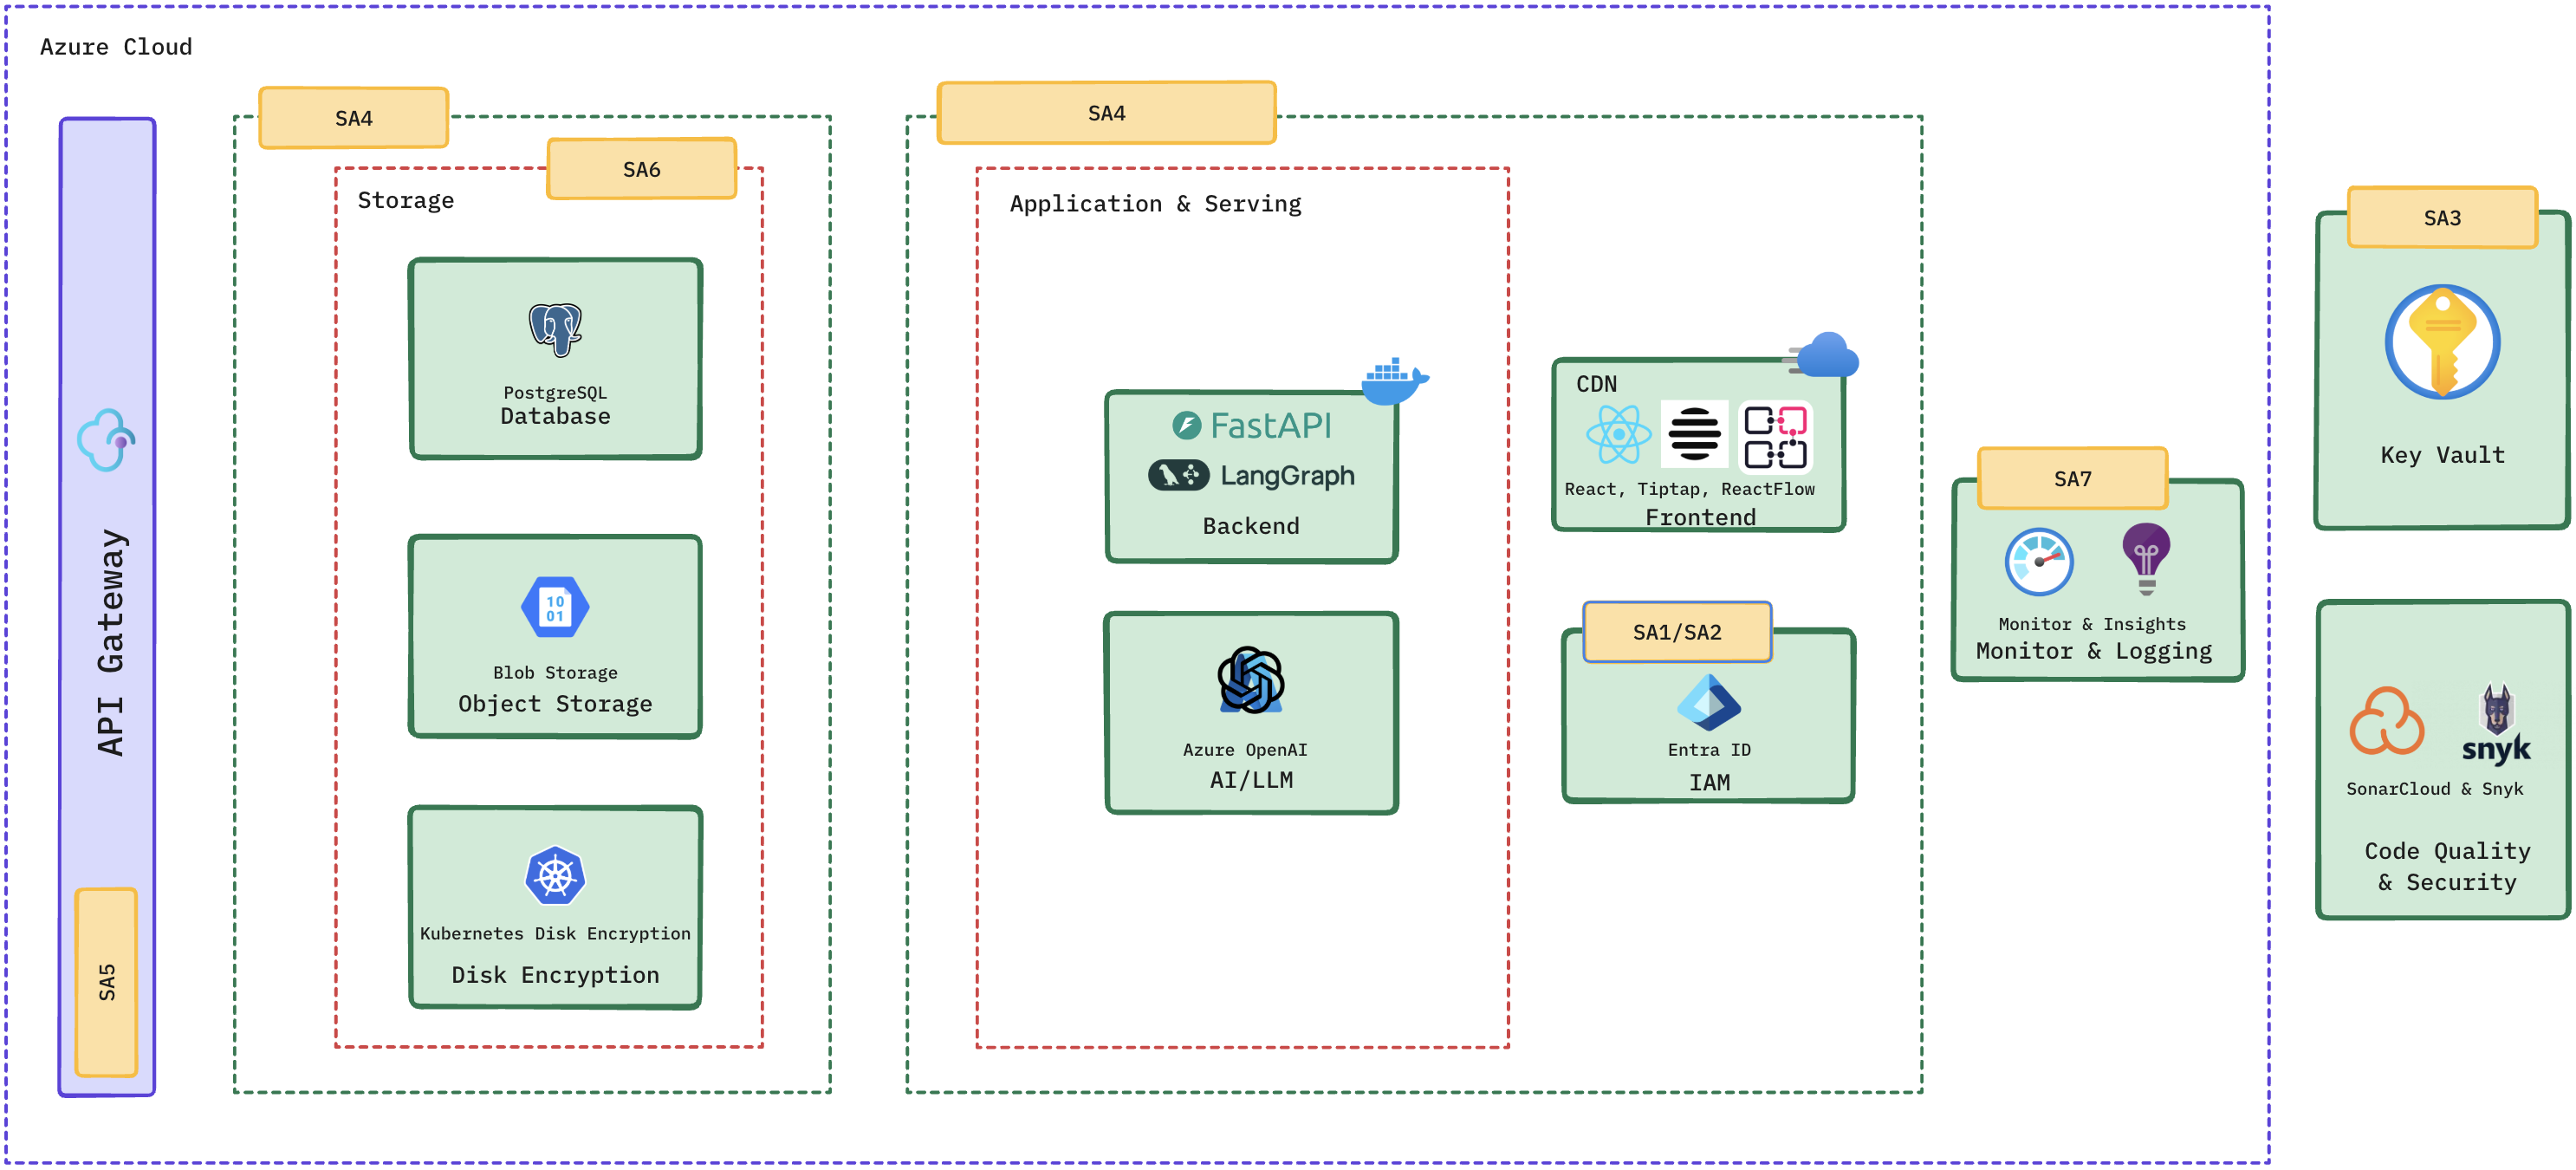
\includegraphics[width=1\textwidth]{Images/Security Architecture.png}
    \captionof{figure}{Security Architecture Overview}
    \label{fig:security_architecture}
\end{center}

Core security practices include robust user authentication and role-based access control via Azure Entra ID, secure management of sensitive credentials and certificates with Azure Key Vault, and network security measures using Virtual Networks and private endpoints. APIs are secured through OAuth 2.0 and TLS encryption, reinforced by API gateway rate limiting. Data security is assured with encryption in transit and at rest, applying stringent access controls and row-level security. The infrastructure’s security compliance and real-time monitoring capabilities are bolstered by Azure Monitor and Application Insights, aligning with industry standards and regulatory requirements.

% Deployment Architecture
\subsection{Deployment Architecture}
The deployment architecture focuses on automating the continuous integration and continuous deployment (CI/CD) processes, ensuring reliability and efficiency in software delivery. The detailed deployment pipeline is represented in Figure \ref{fig:deployment_architecture}.

\begin{center}
    \centering
    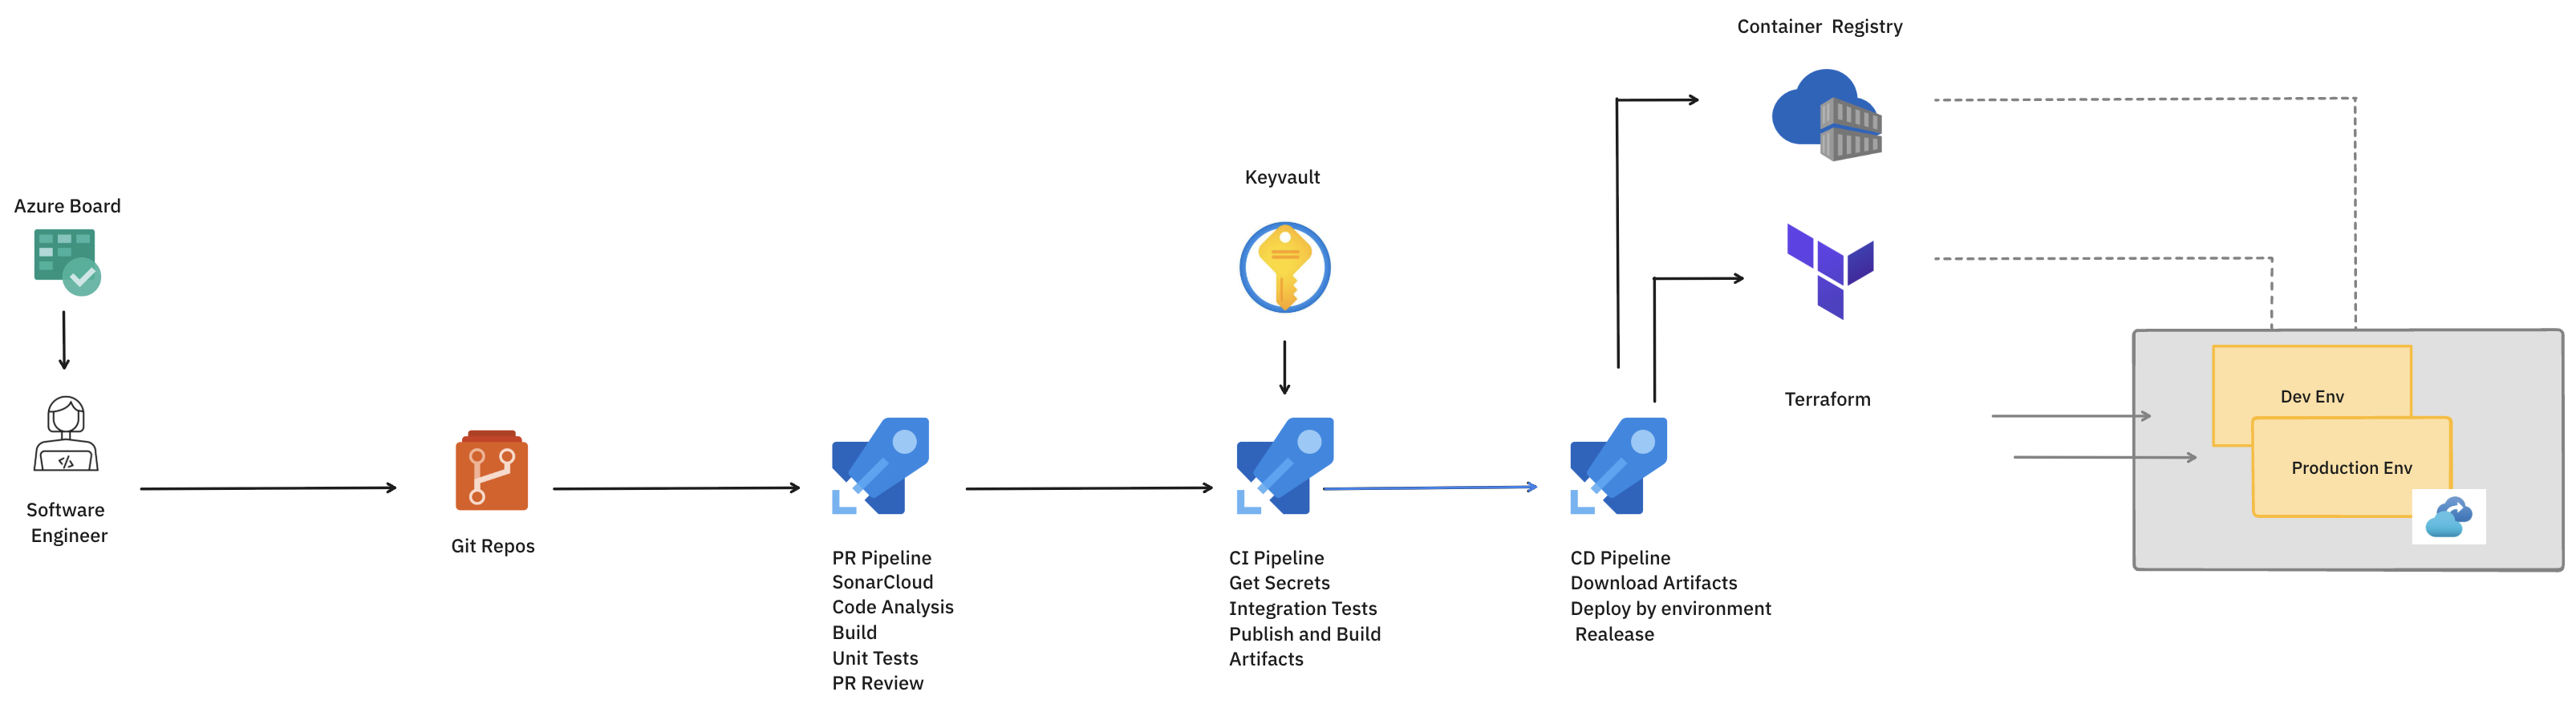
\includegraphics[width=1\textwidth]{Images/Deployment Architecture.png}
    \captionof{figure}{Deployment Architecture Overview}
    \label{fig:deployment_architecture}
\end{center}

The source code, managed in Azure Repos, initiates automated pipelines upon merges. Continuous Integration encompasses code compilation, testing, and security scanning. Docker containers are utilized for application packaging, with container images securely stored in Azure Container Registry (ACR). Continuous deployment uses Helm charts to orchestrate deployments on Azure Kubernetes Service (AKS), ensuring zero downtime with rolling updates. Configuration management leverages Azure Key Vault and Terraform for secure and automated infrastructure provisioning. Enhanced monitoring through Azure Application Insights and Datadog supports real-time performance tracking and anomaly detection. Finally, geo-redundancy and comprehensive backup policies ensure high availability, data protection, and disaster recovery capabilities.

% Conclusion
\section{Conclusion}
This chapter detailed the intelligent contract management platform’s architecture, emphasizing user interactions, frontend/backend components, AI integrations, and specialized legal document management using the Tiptap framework. Comprehensive UML diagrams further clarified component interactions and workflow dynamics. The subsequent chapter will discuss practical implementation and validation, detailing technology choices, implemented functionalities, and verification procedures.